\documentclass[10pt,conference,compsocconf]{IEEEtran}
\usepackage[usenames,dvipsnames]{color}
%\usepackage[english]{babel}
\usepackage{tabularx}
\usepackage{soul}
\usepackage{xparse}
\usepackage{listings}
%\usepackage[normalem]{ulem}



%%%%%%%%%%%%%%%
% Show a list of items "todo" or "done" 
% USAGE: 
% \begin{todolist} 
% 	\todo Something not finished
% 	\done Something finished
% \end{todolist} 
\newenvironment{todolist}{%
  \begin{list}{}{}% whatever you want the list to be
  \let\olditem\item
  \renewcommand\item{\olditem \textcolor{red}{(TODO)}: }
  \newcommand\todo{\olditem \textcolor{red}{(TODO)}: }
   \newcommand\done{\olditem \textcolor{ForestGreen}{(DONE)}: }
}{%
  \end{list}
} 
%%%%%%%%%%%%%%%

%%%%%%%%%%%%%%%
% Show a Author's Note
% USAGE: 
% \incomplete[Optional footnote message to further clarify note]{The text which is currently not finished}
\DeclareDocumentCommand \incomplete{ o m }
{%
\IfNoValueTF {#1}
{\textcolor{red}{Incomplete: \ul{#2}}} 
{\textcolor{red}{Incomplete: \ul{#2}}\footnote{Comment: #1}}%
}
%%%%%%%%%%%%%%%



%%%%%%%%%%%%%%%
% Show a Author's Note
% USAGE: 
% \authnote[Optional footnote message to further clarify note]{The note to your readers}
\DeclareDocumentCommand \authnote { o m }
{%
\IfNoValueTF {#1}
{\textcolor{blue}{Author's Note: \ul{#2}}} 
{\textcolor{blue}{Author's Note: \ul{#2}}\footnote{Comment: #1}}%
}
%%%%%%%%%%%%%%%



%%%%%%%%%%%%%%%
% Strike out text that doesn't belong in the paper
% USAGE: 
% \strike[Optional footnote to state why it doesn't belong]{Text to strike out}
\DeclareDocumentCommand \strike { o m }
{%
\setstcolor{Red}
\IfNoValueTF {#1}
{\textcolor{Gray}{\st{#2}}} 
{\textcolor{Gray}{\st{#2}}\footnote{Comment: #1}}%
}
%%%%%%%%%%%%%%%

\definecolor{light-gray}{gray}{0.95}

\newcommand{\cbox}[3]{
\ \\
\fcolorbox{#1}{#2}{
\parbox{\textwidth}{
#3
}
}
}

% Setup an environment similar to verbatim but which will highlight any bash commands we have
\lstnewenvironment{unixcmds}[0]
{
%\lstset{language=bash,frame=shadowbox,rulesepcolor=\color{blue}}
\lstset{ %
language=sh,		% Language
basicstyle=\ttfamily,
backgroundcolor=\color{light-gray}, 
rulecolor=\color{blue},
%frame=tb, 
columns=fullflexible,
%framexrightmargin=-.2\textwidth,
linewidth=0.8\textwidth,
breaklines=true,
%prebreak=/, 
  prebreak = \raisebox{0ex}[0ex][0ex]{\ensuremath{\hookleftarrow}},
%basicstyle=\footnotesize,       % the size of the fonts that are used for the code
%numbers=left,                   % where to put the line-numbers
%numberstyle=\footnotesize,      % the size of the fonts that are used for the line-numbers
%stepnumber=2,                   % the step between two line-numbers. If it's 1 each line 
                                % will be numbered
%numbersep=5pt,                  % how far the line-numbers are from the code
showspaces=false,               % show spaces adding particular underscores
showstringspaces=false,         % underline spaces within strings
showtabs=false,                 % show tabs within strings adding particular underscores
frame=single,	                % adds a frame around the code
tabsize=2,	                % sets default tabsize to 2 spaces
captionpos=b,                   % sets the caption-position to bottom
breakatwhitespace=false,        % sets if automatic breaks should only happen at whitespace
}
} { }

% Setup an environment similar to verbatim but which will highlight any bash commands we have
\lstnewenvironment{cppcode}[1]
{
%\lstset{language=bash,frame=shadowbox,rulesepcolor=\color{blue}}
\lstset{ %
	backgroundcolor=\color{light-gray}, 
	rulecolor=\color[rgb]{0.133,0.545,0.133},
	tabsize=4,
	language=[GNU]C++,
%	basicstyle=\ttfamily,
        basicstyle=\scriptsize,
        upquote=true,
        aboveskip={1.5\baselineskip},
        columns=fullflexible,
        %framexrightmargin=-.1\textwidth,
       %framexleftmargin=6mm,
        showstringspaces=false,
        extendedchars=true,
        breaklines=true,
        prebreak = \raisebox{0ex}[0ex][0ex]{\ensuremath{\hookleftarrow}},
        frame=single,
        showtabs=false,
        showspaces=false,
        showstringspaces=false,
        numbers=left,                   % where to put the line-numbers
	numberstyle=\footnotesize,      % the size of the fonts that are used for the line-numbers
	stepnumber=4,                   % the step between two line-numbers. If it's 1 each line 
                                % will be numbered
	firstnumber=#1,
         numbersep=5pt,                  % how far the line-numbers are from the code
        identifierstyle=\ttfamily,
        keywordstyle=\color[rgb]{0,0,1},
        commentstyle=\color[rgb]{0.133,0.545,0.133},
        stringstyle=\color[rgb]{0.627,0.126,0.941},
}
} { }

% Setup an environment similar to verbatim but which will highlight any bash commands we have
\lstnewenvironment{mcode}[1]
{
\lstset{ %
	backgroundcolor=\color{light-gray}, 
	rulecolor=\color[rgb]{0.133,0.545,0.133},
	tabsize=4,
	language=Matlab,
%	basicstyle=\ttfamily,
        basicstyle=\scriptsize,
        upquote=true,
        aboveskip={1.5\baselineskip},
        columns=fullflexible,
        %framexrightmargin=-.1\textwidth,
       %framexleftmargin=6mm,
        showstringspaces=false,
        extendedchars=true,
        breaklines=true,
        prebreak = \raisebox{0ex}[0ex][0ex]{\ensuremath{\hookleftarrow}},
        frame=single,
        showtabs=false,
        showspaces=false,
        showstringspaces=false,
        numbers=left,                   % where to put the line-numbers
	numberstyle=\footnotesize,      % the size of the fonts that are used for the line-numbers
	stepnumber=4,                   % the step between two line-numbers. If it's 1 each line 
                                % will be numbered
	firstnumber=#1,
         numbersep=5pt,                  % how far the line-numbers are from the code
        identifierstyle=\ttfamily,
        keywordstyle=\color[rgb]{0,0,1},
        commentstyle=\color[rgb]{0.133,0.545,0.133},
        stringstyle=\color[rgb]{0.627,0.126,0.941},
}
} { }

\newcommand{\inputmcode}[1]{%
\lstset{ %
	backgroundcolor=\color{light-gray},  %
	rulecolor=\color[rgb]{0.133,0.545,0.133}, %
	tabsize=4, %
	language=Matlab, %
%	basicstyle=\ttfamily,
        basicstyle=\scriptsize, %
        %        upquote=true,
        aboveskip={1.5\baselineskip}, %
        columns=fullflexible, %
        %framexrightmargin=-.1\textwidth,
       %framexleftmargin=6mm,
        showstringspaces=false, %
        extendedchars=true, %
        breaklines=true, %
        prebreak = \raisebox{0ex}[0ex][0ex]{\ensuremath{\hookleftarrow}}, %
        frame=single, %
        showtabs=false, %
        showspaces=false, %
        showstringspaces=false,%
        numbers=left,                   % where to put the line-numbers
	numberstyle=\footnotesize,      % the size of the fonts that are used for the line-numbers
	stepnumber=4,                   % the step between two line-numbers. If it's 1 each line 
                                % will be numbered
         numbersep=5pt,                  % how far the line-numbers are from the code
        identifierstyle=\ttfamily, %
        keywordstyle=\color[rgb]{0,0,1}, %
        commentstyle=\color[rgb]{0.133,0.545,0.133}, %
        stringstyle=\color[rgb]{0.627,0.126,0.941} %
}
\lstinputlisting{#1}%
}

%\lstset{ %
%	backgroundcolor=\color{light-gray}, 
%	rulecolor=\color[rgb]{0.133,0.545,0.133},
%	tabsize=4,
%	language=Matlab,
%%	basicstyle=\ttfamily,
%        basicstyle=\scriptsize,
%        upquote=true,
%        aboveskip={1.5\baselineskip},
%        columns=fullflexible,
%        %framexrightmargin=-.1\textwidth,
%       %framexleftmargin=6mm,
%        showstringspaces=false,
%        extendedchars=true,
%        breaklines=true,
%        prebreak = \raisebox{0ex}[0ex][0ex]{\ensuremath{\hookleftarrow}},
%        frame=single,
%        showtabs=false,
%        showspaces=false,
%        showstringspaces=false,
%        numbers=left,                   % where to put the line-numbers
%	numberstyle=\footnotesize,      % the size of the fonts that are used for the line-numbers
%	stepnumber=4,                   % the step between two line-numbers. If it's 1 each line 
%                                % will be numbered
%	firstnumber=#1,
%         numbersep=5pt,                  % how far the line-numbers are from the code
%        identifierstyle=\ttfamily,
%        keywordstyle=\color[rgb]{0,0,1},
%        commentstyle=\color[rgb]{0.133,0.545,0.133},
%        stringstyle=\color[rgb]{0.627,0.126,0.941},
%}


\newcommand{\Laplacian}[1]{\nabla^2 #1}

% set of all nodes received and contained on GPU
\newcommand{\setAllNodes}[0]{\mathcal{G}}
% set of stencil centers on GPU
\newcommand{\setCenters}[0]{\mathcal{Q}}
% set of stencil centers with nodes in \setDepend
\newcommand{\setBoundary}[0]{\mathcal{B}}
% set of nodes received by other GPUs
\newcommand{\setDepend}[0]{\mathcal{R}}
% set of nodes sent to other GPUs
\newcommand{\setProvide}[0]{\mathcal{O}}


\newcommand{\toprule}[0]{\hline}
\newcommand{\midrule}[0]{\hline\hline}
\newcommand{\bottomrule}[0]{\hline}

\newcolumntype{C}{>{\centering\arraybackslash}b{1in}}
\newcolumntype{L}{>{\flushleft\arraybackslash}b{1.5in}}
\newcolumntype{R}{>{\flushright\arraybackslash}b{1.5in}}
\newcolumntype{D}{>{\flushright\arraybackslash}b{2.0in}}
\newcolumntype{E}{>{\flushright\arraybackslash}b{1.0in}}

\DeclareSymbolFont{AMSb}{U}{msb}{m}{n}
\DeclareMathSymbol{\N}{\mathbin}{AMSb}{"4E}
\DeclareMathSymbol{\Z}{\mathbin}{AMSb}{"5A}
\DeclareMathSymbol{\R}{\mathbin}{AMSb}{"52}
\DeclareMathSymbol{\Q}{\mathbin}{AMSb}{"51}
\DeclareMathSymbol{\PP}{\mathbin}{AMSb}{"50}
\DeclareMathSymbol{\I}{\mathbin}{AMSb}{"49}
%\DeclareMathSymbol{\C}{\mathbin}{AMSb}{"43}

%%%%%% VECTOR NORM: %%%%%%%
\newcommand{\vectornorm}[1]{\left|\left|#1\right|\right|}
\newcommand{\vnorm}[1]{\left|\left|#1\right|\right|}
\newcommand{\by}[0]{\times}
\newcommand{\vect}[1]{\mathbf{#1}}
%\newcommand{\mat}[1]{\mathbf{#1}} 

%\renewcommand{\vec}[1]{ \textbf{#1} }
%%%%%%%%%%%%%%%%%%%%%%

%%%%%%% THM, COR, DEF %%%%%%%
%\newtheorem{theorem}{Theorem}[section]
%\newtheorem{lemma}[theorem]{Lemma}
%\newtheorem{proposition}[theorem]{Proposition}
%\newtheorem{corollary}[theorem]{Corollary}
%\newenvironment{proof}[1][Proof]{\begin{trivlist}
%\item[\hskip \labelsep {\bfseries #1}]}{\end{trivlist}}
%\newenvironment{definition}[1][Definition]{\begin{trivlist}
%\item[\hskip \labelsep {\bfseries #1}]}{\end{trivlist}}
%\newenvironment{example}[1][Example]{\begin{trivlist}
%\item[\hskip \labelsep {\bfseries #1}]}{\end{trivlist}}
%\newenvironment{remark}[1][Remark]{\begin{trivlist}
%\item[\hskip \labelsep {\bfseries #1}]}{\end{trivlist}}
%\newcommand{\qed}{\nobreak \ifvmode \relax \else
%      \ifdim\lastskip<1.5em \hskip-\lastskip
%      \hskip1.5em plus0em minus0.5em \fi \nobreak
%      \vrule height0.75em width0.5em depth0.25em\fi}
%%%%%%%%%%%%%%%%%%%%%%

%
%\usepackage[algochapter]{algorithm2e}
%\usepackage[usenames]{color}
% colors to show the corrections
\newcommand{\red}[1]{\textbf{\textcolor{red}{#1}}}
\newcommand{\blue}[1]{\textbf{\textcolor{blue}{#1}}}
\newcommand{\cyan}[1]{\textbf{\textcolor{cyan}{#1}}}
\newcommand{\green}[1]{\textbf{\textcolor{green}{#1}}}
\newcommand{\magenta}[1]{\textbf{\textcolor{magenta}{#1}}}
\newcommand{\orange}[1]{\textbf{\textcolor{orange}{#1}}}
%%%%%%%%%% DK DK
% comments between authors
\newcommand{\toall}[1]{\textbf{\green{@@@ All: #1 @@@}}}
\newcommand{\toevan}[1]{\textbf{\red{*** Evan: #1 ***}}}
%\newcommand{\toevan}[1]{}  % USE FOR FINAL VERSION
\newcommand{\toe}[1]{\textbf{\red{*** Evan: #1 ***}}}
%\newcommand{\toe}[1]{\textbf{\red{*** Evan: #1 ***}}}
\newcommand{\tog}[1]{\textbf{\blue{*** Gordon: #1 ***}}}
%\newcommand{\togordon}[1]{\textbf{\blue{*** Gordon: #1 ***}}}

\renewcommand{\ge}[3]{{\textcolor{blue}{\strike{#1} #2}}\red{(#3)}}
%\renewcommand{\ge}[3]{{\textcolor{blue}{*** \textbf{Gordon:}\strike{#1} #2 ***}}\red{(#3)}}

\newcommand{\gea}[3]{{\textcolor{blue}{\textbf{(Accepted) Gordon:}\strike{#1} #2}}\red{(#3)}}
%\newcommand{\gea}[3]{{\textcolor{blue}{*** \textbf{(Accepted) Gordon:}\strike{#1} #2 ***}}\red{(#3)}}

\newcommand{\eb}[3]{{\textcolor{ForestGreen}{\strike{#1} #2}}\red{(#3)}}
%\newcommand{\eb}[3]{{\textcolor{ForestGreen}{*** \textbf{Evan:}\strike{#1} #2 ***}}\red{(#3)}}

%\def\ge#1#2#3{}{\textbf{\blue{*** Gordon: #2 ***}}}{(#3)}
\newcommand{\gee}[1]{{\bf{\blue{{\em #1}}}}}
\newcommand{\old}[1]{}
\newcommand{\del}[1]{***#1*** }



% \DeclareMathOperator{\Sample}{Sample}
%\let\vaccent=\v % rename builtin command \v{} to \vaccent{}
%\renewcommand{\vec}[1]{\ensuremath{\mathbf{#1}}} % for vectors
\newcommand{\gv}[1]{\ensuremath{\mbox{\boldmath$ #1 $}}} 
% for vectors of Greek letters
\newcommand{\uv}[1]{\ensuremath{\mathbf{\hat{#1}}}} % for unit vector
\newcommand{\abs}[1]{\left| #1 \right|} % for absolute value
\newcommand{\avg}[1]{\left< #1 \right>} % for average
\let\underdot=\d % rename builtin command \d{} to \underdot{}
\renewcommand{\d}[2]{\frac{d #1}{d #2}} % for derivatives
\newcommand{\dd}[2]{\frac{d^2 #1}{d #2^2}} % for double derivatives
\newcommand{\pd}[2]{\frac{\partial #1}{\partial #2}} 
% for partial derivatives
\newcommand{\pdd}[2]{\frac{\partial^2 #1}{\partial #2^2}} 
\newcommand{\pdda}[3]{\frac{\partial^2 #1}{\partial #2 \partial #3}} 
% for double partial derivatives
\newcommand{\pdc}[3]{\left( \frac{\partial #1}{\partial #2}
 \right)_{#3}} % for thermodynamic partial derivatives
\newcommand{\ket}[1]{\left| #1 \right>} % for Dirac bras
\newcommand{\bra}[1]{\left< #1 \right|} % for Dirac kets
\newcommand{\braket}[2]{\left< #1 \vphantom{#2} \right|
 \left. #2 \vphantom{#1} \right>} % for Dirac brackets
\newcommand{\matrixel}[3]{\left< #1 \vphantom{#2#3} \right|
 #2 \left| #3 \vphantom{#1#2} \right>} % for Dirac matrix elements
\newcommand{\grad}[1]{\gv{\nabla} #1} % for gradient
\let\divsymb=\div % rename builtin command \div to \divsymb
\renewcommand{\div}[1]{\gv{\nabla} \cdot #1} % for divergence
\newcommand{\curl}[1]{\gv{\nabla} \times #1} % for curl
\let\baraccent=\= % rename builtin command \= to \baraccent
\renewcommand{\=}[1]{\stackrel{#1}{=}} % for putting numbers above =
\newcommand{\diffop}[1]{\mathcal{L}#1}
\newcommand{\boundop}[1]{\mathcal{B}#1}
\newcommand{\rvec}[0]{{\bf r}}

\newcommand{\Interior}[0]{\Omega}
\newcommand{\domain}[0]{\Omega}
%\newcommand{\Boundary}[0]{\partial \Omega}
\newcommand{\Boundary}[0]{\Gamma}

\newcommand{\on}[1]{\hskip1.5em \textrm{ on } #1}

\newcommand{\gemm}{\texttt{GEMM}}
\newcommand{\trmm}{\texttt{TRMM}}
\newcommand{\gesvd}{\texttt{GESVD}}
\newcommand{\geqrf}{\texttt{GEQRF}}


\newcommand{\minitab}[2][l]{\begin{tabular}{#1}#2\end{tabular}}
\newcommand{\comm}[1]{\textcolor{red}{\textit{#1}}}

\newcommand{\nfrac}[2]{
\nicefrac{#1}{#2}
%\frac{#1}{#2}
}
 % color is defined in macros or misc_mac
% Rename  this file          misc_mac.tex
%----------------------------------------------------------------------
%%%%%%%%%%%%%%%%%%%%%%%%%%%%%%%%%%%%%%%%%%%%%%%%%%%%%%%%%%%%%%%%%%%%%%%%%%%%%%%
%
%	Math Symbols   Math Symbols   Math Symbols   Math Symbols   
%
%%%%%%%%%%%%%%%%%%%%%%%%%%%%%%%%%%%%%%%%%%%%%%%%%%%%%%%%%%%%%%%%%%%%%%%%%%%%%%%
\def\pmb#1{\setbox0=\hbox{$#1$}%
	\kern-.025em\copy0\kern-\wd0
	\kern.05em\copy0\kern-\wd0
	\kern-.025em\raise.0433em\box0}
\def\pmbf#1{\pmb#1}
\def\bfg#1{\pmb#1}

% BETTER VALUES FOR AUTOMATIC FIGURE PLACEMENT THAN THOSE PROVIDED BY 
% LATEX DEFAULTS.

\renewcommand{\textfloatsep}{1ex}
\renewcommand{\floatpagefraction}{0.9}
\renewcommand{\intextsep}{1ex}
\renewcommand{\topfraction}{.9}
\renewcommand{\bottomfraction}{.9}
\renewcommand{\textfraction}{.1}

% #1  position of floating figure (h|t|b|p)
% #1  EPS postscript file
% #2  size
% #3  caption

%usage of newfig:
%  \newfig{file.ps}{3in}{Fig1: this is a figure}

\input{epsf}
\def\newfig#1#2#3#4{
  \begin{figure}[htbp]
  \centering
  \vspace{1ex}
   \includegraphics[width=#2]{#1}
  %\setlength{\epsfxsize}{#2}
  \vspace{-.1in}\caption{\small #3}\break\vspace{.2in}
  \label{#4}
  \end{figure}
}

\def\herefig#1#2#3#4{
  \begin{figure}[h]
  \centering
  \vspace{1ex}
   \includegraphics[width=#2\textwidth]{#1}
  %\setlength{\epsfxsize}{#2}
  \vspace{-.1in}\caption{\small #3}\break\vspace{.2in}
  \label{#4}
  \end{figure}
}


%usage of newfigtwo: 2 figures, vertically stacked
% \newfig
%	{file1.ps}
%	{file2.ps}
%	{width}
%	{vertical space}
%	{Caption}

\def\newfigtwo#1#2#3#4#5{
  \begin{figure}[htbp]
  \vspace{1ex}
  \setlength{\epsfxsize}{#3}
  \centerline{\epsfbox{#1}}
  \vspace{#4}
  \setlength{\epsfxsize}{#3}
  \centerline{\epsfbox{#2}}
  \vspace{-.1in}\caption{\small #5}\break\vspace{.2in}
  \label{#1}
  \end{figure}
}

\def\newfigh#1#2#3#4{  % add height specification
  \begin{figure}[htbp]
  \vspace{1ex}
  \setlength{\epsfxsize}{#2}
  \setlength{\epsfysize}{#4}
  \centerline{\epsfbox{#1}}
  \vspace{-.1in}\caption{\small #3}\break\vspace{.2in}
  \label{#1}
  \end{figure}
}

\def\etal{{{\em et~al.\,\,}}}
\def\note#1{\\ =====#1===== \\}
\def\FBOX#1{\ \\ \fbox{\begin{minipage}{5in}#1\end{minipage}}\\ }
\newcount\sectionno     \sectionno=0
\newcount\eqnum         \eqnum=0
\def\addeqno{\global\advance \eqnum by  1 }
\def\subeqno{\global\advance \eqnum by -1 }
%\def\eqn{\addeqno \eqno \hbox{(\number\sectionno.\number\eqnum)} }

\def\tildetilde#1{\tilde{\tilde{#1}}}
\def\barbar#1{\overbar{\overbar{#1}}}

\def\vsp#1{\vspace{#1 ex}}
\def\fpar{\hspace{\parindent}}
%
%  \pf : 2 arguments: numerator and denominator of partial derivative
%
\def\pf#1#2{{\frac{\partial{#1}}{\partial{#2}}}}
\def\pfs#1#2{{\partial_{#2}{#1}}}
\def\pftwo#1#2{{\frac{\partial^2{#1}}{\partial{#2}^2}}}
\def\pfxx#1#2{{\frac{\partial^2{#1}}{\partial{#2}^2}}}
%\def\pfxy#1#2{{\frac{\partial^2{#1}}{\partial{#2}\partial{#3}}}}
\def\pfn#1#2#3{{\frac{\partial^{#1}{#2}}{\partial{#3}^{#1}}}}
\def\df#1#2{{\frac{d{#1}}{d{#2}}}}
\def\dfn#1#2#3{{\frac{d^{#1}{#2}}{d{#3}^{#1}}}}
\def\Dt#1#2{\frac{D#1}{D#2}}
\def\dt#1#2{\frac{d#1}{d#2}}
\def\bld#1{{\bf #1}}
\def\pfp#1#2#3{\pf{}{#3}{\left(\frac{#1}{#2}\right)}}

\def\norm#1{\|#1\|}

%
% Graphic characters  (\dot already defined by TeX/LateX)
%
\def\dash{\rule[1.5pt]{2mm}{.3mm}\HS{.9mm}}
\def\dott{\rule[1.5pt]{.7mm}{.3mm}\HS{.7mm}}
\def\dashline{\dash\dash\dash}
\def\dotline{\dott\dott\dott\dott\dott\dott}
\def\dashdotline{\dash$\cdot$\HS{.9mm}\dash}
\def\solidline{\rule[2pt]{7mm}{.3mm}}
% 
% overcircle
%
\def\ovcircle#1{\buildrel{\circ}\over{#1}}
%\def\below#1#2{\buildrel{#2}\under{#1}}
%\def\above#1#2{\buildrel{#2}\over{#1}}
%
%  big parenthesis and brackets
%
\def\bigpar#1#2{{\left(\frac{#1}{#2}\right)}}
\def\bigbra#1#2{{\left\[\frac{#1}{#2}\right\]}}

\def\Lp{\left(}
\def\Rp{\right)}
\def\Lb{\left[}
\def\Rb{\right]}
\def\Ln{\left\langle}
\def\Rn{\right\rangle}
\def\Ld{\left.}
\def\Rd{\right.}
\def\Lv{\left|}
\def\Rv{\right|}
\def\Lbr{\left|}
\def\Rbr{\right|}
\def\lng{\langle}
\def\rng{\rangle}
\def\Lc{\left\{}
\def\Rc{\right\}}
%%% %

% Cannot be handled by Lyx
%\def\[{{[}}
%\def\]{{]}}

%
\def\eol{\nonumber \\}
\def\eolnonb{\nonumber\\}
\def\eolnb{\\}
\def\nonb{\nonumber}
\def\be{\begin{equation}}
\def\ee{\end{equation}}
\def\BEQNA{\begin{eqnarray}}
\def\EEQNA{\end{eqnarray}}
\def\eqa{&=&}
\def\beqna{\begin{eqnarray}}
\def\eeqna{\end{eqnarray}}
\def\bverb{\begin{verbatim}}
\def\everb{\end{verbatim}}
\def\VERB#1{\bverb #1 \everb}
\def\btbl{\begin{tabular}}
\def\etbl{\end{tabular}}
\def\bmini{\begin{minipage}[t]{5.5in}}
\def\emini{\end{minipage}}
\def\parray#1#2{\left(\!\!\!\begin{array}{#1}#2\end{array}\!\!\!\right)}
\def\barray#1#2{\left[\begin{array}{#1}#2\end{array}\right]}
\def\carray#1#2{\left\{\begin{array}{#1}#2\end{array}\right.}
\def\darray#1#2{\left|\begin{array}{#1}#2\end{array}\right|}

\def\BEGTABLE#1{\begin{table}[hbt]\vspace{2ex}\begin{center}\bmini\centering\btbl{#1}}
\def\ENDTABLE#1#2{\etbl\caption[#1]{#2}\EMINI\end{center}\vspace{2ex}\end{table}}

\def\bfltbl#1{\begin{table}[hbt]\vspace{2ex}\begin{center}\bmini\centering\btbl{#1}}
\def\efltbl#1#2{\etbl\caption[#1]{#2}\emini\end{center}\vspace{2ex}\end{table}}
\def\mcol{\multicolumn}
%
%  label equations with (#)
%
\def\reff#1{(\ref{#1})}
%
%  macros borrowed from viewgraph package
%

\newenvironment{LETTRS}[3]{\begin{letter}{#1}
\input{origin}\opening{Dear #2:}\input{#3}\closing{Sincerely yours,}\end{letter}}{\clearpage}

\newenvironment{VIEW}[1]{{\BC\Huge\bf #1 \EC}\LARGE\VS{.05in}}{\clearpage}

\def\RM#1{\rm{#1\ }}
\def\BV{\begin{VIEW}}
\def\EV{\end{VIEW}}

\def\NI{\noindent}

\def\VS{\vspace*}
\def\HS{\hspace*}
\def\IT{\item}

\def\BARR{\begin{array}}
\def\EARR{\end{array}}

\def\BPARR{\left(\begin{array}}
\def\EPARR{\end{array}\right)}

\def\BDET{\left|\begin{array}}
\def\EDET{\end{array}\right|}

\def\BDF{\begin{definition}}
\def\EDF{\end{definition}}

\def\BSU{\begin{block}{Summary}}
\def\ESU{\end{block}}

\def\BEX{\begin{example}}
\def\EEX{\end{example}}

\def\BTH{\begin{theorem}}
\def\ETH{\end{theorem}}

\def\BCO{\begin{corollary}}
\def\ECO{\end{corollary}}

\def\BPROOF{\begin{proof}}
\def\EPROOF{\end{proof}}

\def\BLM{\begin{lemma}}
\def\ELM{\end{lemma}}

\def\BEQ{\begin{equation}}
\def\EEQ{\end{equation}}

\def\BEQNNB{$$}
\def\EEQNNB{$$}

\def\BE{\begin{enumerate}}
\def\EE{\end{enumerate}}

\def\BD{\begin{description}}
\def\ED{\end{description}}

\def\BI{\begin{itemize}}
\def\EI{\end{itemize}}

\def\BC{\begin{center}}
\def\EC{\end{center}}

\def\BFIG{\begin{figure}}
\def\EFIG{\end{figure}}

\def\BTABB{\begin{tabbing}}
\def\ETABB{\end{tabbing}}

\def\BMINI{\begin{minipage}}
\def\EMINI{\end{minipage}}

\def\BTABLE{\begin{table}}
\def\ETABLE{\end{table}}

\def\BTABUL{\begin{tabular}}
\def\ETABUL{\end{tabular}}

\def\MCOL{\multicolumn}
\def\UL{\underline}
\def\ULL#1{\UL{\UL{#1}}}

\def\BDOC{\begin{document}}
\def\EDOC{\end{document}}

\def\EM#1{{\em #1\/}}
\def\FN{\footnote}

% Courtesy of Ugo Piomelli

\def\latexfig #1 #2 #3 #4 #5 {\ \vfill
\hfill\hbox to 0.05in{\vbox to #3truein{
         \special{psfile="#1" angle=270 hscale=100 
                  hoffset=#4 voffset=#5 vscale=100} }\hfill}
\hfill\vspace{-0.1in}        }

% #1 is the .ps filename
% #2 is not used in the present version
% #3 is the size of the white space left above the caption (in inches)
% #4 is the horizontal offset from some unknown reference point.
%    It is in 1/72 of an inch and is positive to the right.
% #5 is the vertical offset from some unknown reference point.
%    It is in 1/72 of an inch and is positive upwards.


% Rename this file:    setupicase.tex
%----------------------------------------------------------------------
\setlength{\textwidth}{6.5in}
\setlength{\textheight}{9.0in}
\setlength{\topmargin}{-.1875pt}
\setlength{\oddsidemargin}{0pt}
\setlength{\evensidemargin}{0pt}
\setlength{\headsep}{0pt}
\setlength{\parskip}{1ex}
\setlength{\headheight}{0pt}



\def\red#1{\textbf{\textcolor{red}{#1}}}
\def\blue#1{\textbf{\textcolor{blue}{#1}}}
\def\qes#1{{\blue{*** For Erik: #1 ***}}}
\def\es#1{{\blue{*** For Erik: #1 ***}}}
\def\ge#1{{\red{*** For Gordon: #1 ***}}}
\def\ttt#1{{\tt #1}}
\def\bold#1{{\bf #1}}

\usepackage{soul}
\usepackage{xspace}
\usepackage{color} 
\definecolor{darkgreen}{rgb}{0,0.5,0}
\usepackage[colorlinks=true,% 
  linkcolor=red,% 
  citecolor=darkgreen,%
  urlcolor=blue]{hyperref}

\usepackage{listings}


\newcommand{\todo}[1]{{\color{red}\textbf{\hl{#1}}\xspace}}

\def\qes#1{}
\def\es#1{}
%\def\ge#1{}
%\usepackage{morefloats}

\newcommand{\ceil}[1]{\left\lceil#1\right\rceil}

\usepackage{amsmath}
\usepackage{amssymb}


\usepackage[pdftex]{graphicx}
\usepackage{subfigure}
%\usepackage{fixltx2e}
\usepackage{url}
\hyphenation{op-tical net-works semi-conduc-tor}


\begin{document}
\title{Sparse Matrix Vector Multiplication with Multiple vectors and
  Multiple Matrices on the MIC Architecture}


\author{\IEEEauthorblockN{Gordon Erlebacher\IEEEauthorrefmark{1},
Erik Saule\IEEEauthorrefmark{2}, Natasha Flyer\IEEEauthorrefmark{3}, 
and Evan Bollig\IEEEauthorrefmark{1}}
\IEEEauthorblockA{\IEEEauthorrefmark{1}Department of Scientific Computing, 
Florida State University, Tallahassee, FL 32306-4120\\
Email: gerlebacher@fsu.edu}
\IEEEauthorblockA{\IEEEauthorrefmark{2}Department of Computer Science, University of North Carolina at Charlotte\\
Email: esaule@uncc.edu}
\IEEEauthorblockA{\IEEEauthorrefmark{3}Computational and Information Systems Laboratory, UCAR \\
Email: flyer@ucar.edu}
\IEEEauthorblockA{\IEEEauthorrefmark{4}Department of Scientific Computing, Florida State University\\
Email: bollig@gmail.com}}
\maketitle


\begin{abstract}
In this paper, we develop an efficient scheme for the calculation of
derivatives within the context of Radial Basis Function
Finite-Difference (RBFFD). RBF methods express functions as a linear
combination of radial basis functions on an arbitrary set of
nodes. The Finite-Difference component expresses this combination over
a local set of nodes neighboring the point where the derivative is
sought.  The derivative at all points takes the form of a sparse
matrix/vector multiplication (spmv).

In this paper, we consider the case of local stencils with the number
of nodes at each point and encode the sparse matrix in ELLPACK
format. We increase the number of operations relative to memory
bandwidth by calculating four derivatives of four different functions,
or 16 different derivatives. We demonstrate a novel implementation on
the MIC architecture, taking into account its advanced swizzling and
channel interchange features. We present benchmarks that show an
almost order of magnitude increase in speed compared to efficient
implementations of a single derivative. We explain the results through
consideration of operation count versus memory bandwidth.
\end{abstract}

\begin{IEEEkeywords}
OpenMP; MIC; spmv; sparse matrix; Radial Basis Function;
\end{IEEEkeywords}

\IEEEpeerreviewmaketitle

\section{Introduction}
\cite{Stock12-TACC} is all dense. \cite{
  Molka:2009:MPC:1636712.1637764} is about memory modeling not
directly spmv.

\cite{DBLP:journals/ijhpca/ShantharamCR11,
  DBLP:journals/corr/abs-1101-0091 }

The multiplication of sparse matrix by a dense vector (SpMV) is an
important kernel in many fields from scientific computing~\cite{} to
graph analysis (recommender systems~\cite{Brin98}, graph
drawing~\cite{Koren05}). So improving the performance of SpMV has
captured the interest of many researcher; including the development of
various implementations for multi-core
CPUs~\cite{Buluc2009SPAA,Williams07} and
GPUs~\cite{Bell08, conf/ipps/KreutzerHWFBB12,
  journals/concurrency/VazquezFG11,kumar2012accelerating}. The main
challenge that is faced to obtain good performance for SpMV is that
the operation are conducted using memory location that are irregular
and often unpredictible. That make that the kernels are mostly memory
bound and there is a significant instruction overhead per flop.

Common improvement techniques such as register blocking, bandwidth
reduction (matrix reordering~\cite{Cuthill69}), partitioning to fit in
cache or TLB~\cite{Nishtala07,Temam:1992:CBS:147877.148091,conf/ppsc/Toledo97},
unrolling~\cite{Mellor-Crummey04} have impacts which are very
dependent on the matrix and overall do not lead to dramatic
improvement. (The state-of-the-art techniques in OSKI~\cite{Vuduc05}
provide some useful yet limited improvements). Register blocking~\cite{conf/ppsc/Toledo97} does
not apply well to most the matrix at hand (despite it can be applied
with virtually no overhead in all cases thanks to compressed
representation~\cite{Buluc11}). there is about 8 bytes of the matrix to move
in per non zero (assuming single precision); each nonzero requires two
floating point operations leading to a flop-to-byte ratio of at most
$\frac{1}{4}$. This limits the obtained performance to at most a
quarter of the bandwidth of the architecture wasting a lot of
potentially useful cycles. The commonly used techniques are mostly
designed to reach that bound rather than overcome it.

Fortunately that fate is not inevitable. One solution would be to pair
multiple component of an application to schedule a more instruction
intensive kernel simultaneously with SpMV, relying on some hardware
threading capabilities, such as HyperThreading, to reduce the cycle
wastage. However most ot the applications that use SpMV do not
typically have an instruction intensive kernel to run simultaneously.

An other solution, and the one we pursue in this paper, is to compute
multiple SpMV at once on matrices that have the same sparsity
patterns. Obviously not all the applications have such a property. But
important classes of applications such as graph
recommendation~\cite{}, eigensolving~\cite{} and the computation of
derivative of Radial Basis Functions(RBF)~\cite{} can use multiple
SpMVs simultaneously. In this paper in particular, we investigate the
case of the derivative of RBFs where four derivatives of four
different function is expressed as the multiplication of four vectors
by four matrices with identical sparsity patterns leading to the
simultaneous execution of 16 SpMVs at a time. Using multiple vectors
at a time has been investigated before to densify the
computations~\cite{Im01} but this is the first time that the
densification comes from adding both vectors and matrices.

To perform our analysis, we focus our attention on the improvement
that we can achieve on the Intel Xeon Phi processor. It follow the
Many Integrated Core (MIC) architecture, which has a significant
memory bandwidth and peak flop throughput thanks to its 512-bit large
SIMD registers. The Xeon Phi processor has been shown to be promising
for sparse linear algebra compared to more classical CPU or GPU
architecture~\cite{Saule13-ARXIV, Liu:2013:ESM:2464996.2465013, cramer2012openmp}.

In Section~\ref{sec:rbf} we present the computation of RBFs and how it
can be expressed 16 multiplication of 4 vectors by 4 sparse matrices
with a common sparsity pattern. Section~\ref{sec:model} presents an
estimation of the instruction intensity of various form of the
computations and we show that a 5- to 6- fold improvement can be
expected when computing the 16 multiplications simultaneously and
reach a total of about 200 Gflop/s. This performance represents
approximatively 10\% of the available flop/s of a Knight Corner
coprocessor. Therefore, it is necessary to have implementations that
perform the computation in as little amount of instructions as
possible. We describe in Section~\ref{sec:impl} the details of the MIC
architecture and how to use specialized load, store, swizzle and
permutation instruction to efficiently bring the data in the vector
registers to be processed. Section~\ref{sec:expe} gives some
experimental result about the amount of bandwidth that can be achieved
depending on how the spmv kernel is written and the actual performance
of the various kernel on multiple classes of matrices some generated
for analysis purpose and some extracted from and RBF application. A
performance of xxx GFlop/s is achieved on real scenario. Concluding
remarks and perspectives are provided in Section~\ref{sec:ccl}.

\section{Derivatives of Radial Basis Functions}
\label{sec:rbf}

%In the theory of Radial Basis Functions Finite-Difference (RBFFD),
%derivatives of a function $f(\rvec)$ at node $i$ are expressed as a
%linear combination of the function values at the stencil center and
%the nodes connected to node $i$ (Figure~\ref{fig:rbf_stencils}). Thus
%$y$ is a discrete derivative of the vector $x$.

In this paper, we propose a new idea that is applicable to radial
basis functions (RBFs). Their strength is the ability to randomly
distribute points across complex physical domains, and have an
implementation that is independent of dimensionality. RBFs approximate
a function $f(\xvec)\subset \mathbb{R}^d$ sampled at a set of $N$
distinct point locations, $x_j$, by linearly combining translates of a
single radially symmetric function $\phi(r)$, where $r =
\|\xvec-\xvec_{j}\|$ denotes the Euclidean distance (e.g., in 2-D
$\sqrt{(x-x_j)^2+(y-y_j)^2}$) between where the function is evaluated
$\xvec$ and where the RBF is centered $\xvec_{j}$. That is, the
interpolant is $s(\xvec) = \sum_{j=1}^{N} w_j
\phi_i(\|\xvec-\xvec_{j}\|)$. The weights $w_j$ are obtained by
inverting the system
\begin{equation}
\parray{lccr}{
\phi_{11} & \phi_{12} & \cdots & \phi_{1N} \\
\vdots & \ddots & \vdots & \vdots \\
\phi_{n1} & \phi_{n2} & \cdots & \phi_{NN} 
}
\parray{c}{ w_{1} \\ \vdots \\ w_{N} }
=
\parray{c}{ f(\xvec_1) \\ \vdots\\ f(\xvec_N) }. 
\label{eq:rbf}
\end{equation}
where $\phi_{ij} = \phi(\|\xvec_i-\xvec_j\|)$. 
%\end{equation}
%\begin{equation}
%\begin{bmatrix}
%\phi(\|\xvec_{1}-\xvec_{1}\|) & \phi(\|\xvec_{1}-\xvec_{2}\|) & \cdots & \phi(\|\xvec_{1}-\xvec_{N}\|) \\
%\vdots & \ddots & \vdots  \\
%\phi (\|\xvec_{n}-\xvec_{1}\|) & \phi(\|\xvec_{n}-\xvec_{2}\|) & \cdots & \phi(\|\xvec_{N}-\xvec_{N}\|)
%\end{bmatrix}

The RBF differentiation matrix, $D_N$, is derived by applying the
desired analytic derivative operator $L$ to the RBF interpolant
$s(\xvec)$ above and evaluating it at the point locations. For very
large problems, this is a computationally expensive since the matrix
in (\ref{eq:rbf}) is full and inversion requires O$(N^3)$
operations. To alleviate the cost of this global approach (i.e. using
every node in the domain to calculate the derivative at a given node
$\xvec_i$), RBF-generated finite differences (RBF-FD) have been
derived \cite{TAI1,TAI2,SDY02,WrFo06,FoL11,FLBWSC12}. RBF-FD uses only
a local set of the $n_z-1$ nearest neighbors to the point $\xvec_i$ to
approximate the derivative. In other words,
$Lf(\xvec_i)=\sum_{j=1}^{n_z}a_jf(\xvec_j)$. The differentiation
weights, $a_j$, are calculated by enforcing that this linear
combination should be exact for RBFs,
$\{\phi(\|\xvec-\xvec_{j}\|)\}_{j=1}^{n_z}$, centered at each of the
node locations $\{\xvec_j\}_{j=1}^{n_z}$ (classical finite differences
(FD) would enforce that it be exact for polynomials instead). Similar
to FD, as the stencil size $n_z$ increases so does the order of the
method.

For a total of $N$ points, there will be $N$ linear systems to solve,
each of size $n_z \times n_z$. Each linear solve produces a row of the
RBF-FD differentiation matrix $D_{n_z}$, resulting in a $N \times N$
matrix with $n_zN$ nonzero entries. To evaluate the derivative at all
points in the domain, takes the form
$$
  \mathbf{g} = D_{n_z} \mathbf{f}
$$

where $f$ is the source vector of function values and $g$ is the
resulting vector of derivative values. The computation of a single
derivative has been reduced to a SpMV, where each row has $n_z$
nonzeros. Since the sparsity of each row is constant, ELLPACK~\cite{}
becomes the most appropriate matrix compression scheme\cite{}. In
practice, $n_z=32$ in two-dimensional flows and 64 or 100 for
three-dimensional flows. These numbers are similar to what is used in
finite-element codes. Notice that the non zero elements of the matrix
correspond to a relation of nearest neighbor. This relationship is not
necessarily symmetric as shown in Figure~\ref{fig:rbf_stencils} which
means that the matrix sparsity pattern might not be symmetric either.

\begin{figure}[tbh]
  \centering
  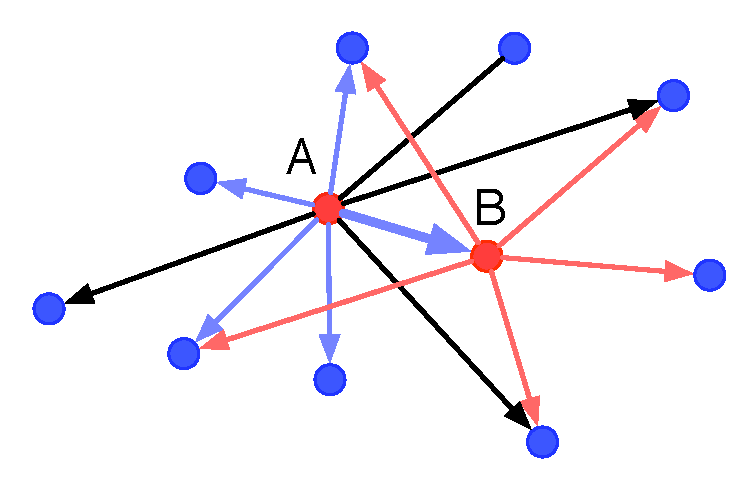
\includegraphics[width=\linewidth]{figures/rbf_stencils.pdf}
  \caption{RBFFD Stencils. Each node of the stencil is connected to
    $n_z-1$ stencil nodes in addition to itself. In the figure, node
    $A$ is connected to $B$, but $B$ is {\em not\/} connected to
    $A$. Thus adjacency graph of $A$ is not-symmetric.}
  \label{fig:rbf_stencils}
\end{figure}

Many problems in fluid dynamics and in the geosciences require the
solution to transport equations of the form
$$
\pf{Q}{t} = f(Q,Q_x, Q_y, Q_z, \Laplacian{Q})
$$
where $Q$ is a vector of unknowns (3 components of velocity, pressure,
temperature). For example, in solving a system of equations, it is
often necessary to compute the $x$ derivative of multiple functions,
typically four for the Euler equations, or five for the Navier-Stokes
equations. Multiple right-hand sides transform a SpMV into a SpMM
(Sparse Matrix/dense Matrix multiplication), which improves register
utilization and decreases cache misses by vectorizing over the
multiple source vectors. Further improvements are possible by
recognizing that different derivative matrices (x,y,z and Laplacian
for example), have the same sparsity distribution; only the weight
change.  Thus, alternative to computing a derivative of multiple
functions, we can calculate multiple derivatives of a single
functions. The increased memory bandwidth due to an increase in the
number of derivative matrices is offset by better cache utilization,
leading to an overall benefit.

% GORDON I WOULD ELIMINATE BELOW AND END HERE.

%**** PUT ELSEWHERE OR ELIMINATE? ****
%
%When solving a one dimensional system of PDEs, one might require an
%$x$ derivative of multiple functions. For example, the Euler equations
%require the $x$ derivative of the three components of velocity and
%pressure. In this case, there are $n_v=4$ vectors $x^k$,
%$k=0,\cdots,3$.
%
%Thus for each vector element $y_i$, we compute $y_i = \sum_j A_{ij}
%x_j$. If $A_i$ is row $i$ of $A$, $y_i$ is simply the dot product $A_i
%x$. The next level of generality is to consider $n_v$ vectors $x^k$,
%$k=0,\cdots,n_v-1$. Whatever the spmv implementation, one achieves
%improved performance if the matrix formed from the columns $x^k$ are
%stored in row major order. Thus, $x^0_0,x^1_0,\cdots,x^{n_v-1}_0$, are
%stored in consecutive memory location. The random access of the
%elements of $x$ is thus reduced. Maximum efficiency is achieved when
%$n_v=16$ floats or $8$ doubles, given that cache lines take 64
%bytes. We will benchmark this case, labeled $Svn$, where $n$ refers to
%the number of vectors (Iv4 uses four vectors). The $S$ refers to singe
%precision. A double precision run is labelled $Dvn$.
%
%Alternatively, when solving a PDE, one might require derivatives of a
%given scalar function with respect to coordinate directions $x$, $y$,
%$z$. Second order operators of often required, such as a second
%derivative with respect to $x$ or a Laplacian operator. In the RBFFD
%formulation, on can compute different derivatives using the same
%stencil, but with different weights. In other words, the adjacency
%matrix that corresponds to $A$ remains constant, but the matrix
%elements of $A$ change with the particular derivative.  In this case,
%label with a superscript $l$ the particular matrix $A^k$. Since the
%adjacency matrix is assumed invariant, there is only need for a single
%matrix \ttt{C{ij}}. In Ellpack format, each row is of constant size
%(the number of nonzeros per row of $A$. $C_{ij}$ is the column number
%that locates the $j^{th}$ nonzero in row $i$ of $A$.
%
%
%\todo{Must rewrite the above to make it more focused on the
% application. Remove the architectural/implementation details such as
%  using ELLPACK. Let's focus on on why this computation is important
%  and how does the 16 multiplication appears in the equations.}



\newfig{figures/matrix_structure.pdf}{\linewidth}{Matrix Structure.}{fig:mat_struct}




\section{Modelization of the Potential Improvements}
\label{sec:model}

We saw in the previous section that one can express the RBF problem as
a multiplication of four matrices by four vectors. We present here an
estimation of the variation on the flop intensity of the computation
and its impact on the expected performance of the
application. Relevant notations are given in Table~\ref{tab:not}.

\begin{figure}
  \begin{center}
    \scalebox{.9}{
      \begin{tabular}{|c|l|}
        %\hline
        %& & \\
        \hline
        $b_i$ & number of bytes per index \\
        $b_x$ & number of bytes per value \\
        $n_z$ & number of nonzeros per row $A$ \\
        $n_r$ & number of column/rows of $A$ \\
        $n_c$ & total number of non-zero\\
        $n_v$ & number of {\tt x} vectors \\
        $n_m$ & number of matrices \\
        $s_M$ & size of the matrice(s) in bytes\\
        $s_x$ & size of the {\tt x} vector(s) in bytes\\
        $s_y$ & size of the {\tt y} vector(s) in bytes\\
        \hline
        $cl$    & size of a cache line in bytes\\
        $b_{wT}$ & number of bytes written to memory  \\
        $b_{rT}$ & minimum number of bytes read from memory  \\
        $b_T$   & minimum number of bytes transferred  \\
        $B_{rT}$ & maximum number of bytes read from memory \\
        $B_T$   & maximum number of bytes transferred  \\
        $O$     & number of floating point operations \\
        $I_b$   & maximal computational intensity\\
        $I_w$   & minimum computational intensity\\        
        \hline
      \end{tabular}
    }
  \end{center}
  \caption{Notations}
  \label{tab:not}
\end{figure}

Each vector in the problem is of dimension $n_r$ and each dimension
tasks $b_x$ bytes. There are $n_v$ {\tt x} vectors and $n_v n_m$ {\tt
  y} vectors, which lead to the size of the {\tt x} and {\tt y} vectors:
$$s_x = n_v b_x n_r$$ $$s_y = n_v n_m b_x n_r$$

The matrix is composed of $n_r$ rows and columns with $n_z$ non-zeros
per row leading to a total of $$n_c = n_r n_z$$ non-zero entries in
the matrix. Each of these non-zero entries has one index of size $b_i$
and $n_m$ values of size $b_x$. The matrices have a total size
of $$s_M = n_c (b_i + b_x n_m) = n_r n_z (b_i + b_x n_m)$$

If we assume an algorithm where the rows are processed one after
the other, the amount of memory written is precisely the
size of the {\tt y} vector. (This assumption removes the possibility of
cache partitioning techniques.) $$b_{wT} = s_y = n_v n_m b_x n_r$$

The amount of data read from memory depends highly on both the algorithm's
execution path, and on %algorithm execute, 
how the matrix is structured. But in the best case
both the matrix $A$ %is read a single time 
and the source vector {\tt x} are read once
%read a single time 
from the main memory. (We assume that all the elements of $\tt x$ are involved
in the SpMV.)  %is used is reasonnable since only oddly shaped matrix will
%left a dimension of the vector unused.) 
Thus, $$b_{rT} = s_M + s_x = n_r n_z
(b_i + b_x n_m) + n_v b_x n_r$$
 $$b_T = b_{rT} + b_{wT} =  n_r n_z (b_i + b_x n_m) + n_v b_x n_r (1 + n_m)$$

Notice that there is no reason for a piece of the matrix to be read
multiple times. But assuming that each element of the {\tt x} vector
is read a single time is a strong assumption. If using a single core,
it assumes that either the cache of the architecture can store the full
{\tt x} vector or that the matrix is sufficiently well structured 
causing no cache trashing. If using multiple core, this assumes that
no element of the {\tt x} vectors will be used by multiple
cores. \cite{Saule12} showed that there is very little cache trashing
in practice, but it showed that having elements of the vectors used by
multiple cores can have a significant impact on the performance
(growing with $n_v$).

On the other hand, in the worst case, every time the {\tt x} vector is
accessed, the value needs to be transfered from memory again. So in
total, there are as many transfers as the number of non-zeros in the
matrix. Note however that most architectures cannot read memory a single 
byte at a time. Instead, a minimum number of bytes,equal to the size o a cacheline, 
are transfered at once. 
%multiple bytes, with each chunk equal to the data do not allow to read the memory
%one byte at a time but always in a set of multiple bytes. On most
%cached architecture, that 
%the minimum size corresponds to the size $cl$ of
%a cacheline (typically 64 bytes). 
When there are multiple
vectors, each non-zero element uses $n_v$ consecutive entries. The
worst case number of bytes read and transfered are 
$$B_{rT} = s_M + n_c cl \ceil{\frac{n_vb_x}{cl}} $$ 
$$B_T = n_v n_m b_x n_r + n_r n_z \left ( b_i + b_x n_m +  cl \ceil{\frac{n_vb_x}{cl}} \right)$$

In SpMV, each non-zero of the matrix requires two floating point
operations: one for performing the multiplication and one for
accumulating the result row-wise. Here we are dealing with $n_v n_m$
simultaneous SpMVs and the number of floating point operations is
$$O = 2 n_v n_m n_c = 2 n_v n_m n_z n_r$$

The computation intensity is the amount of computations performed per
byte transfered. In the worst case and in the best case, we have
$$I_b = \frac{O}{b_T} = \frac{2 n_v n_m}{ (b_i + b_x n_m) + n_v n_m b_x n_z^{-1} + n_v b_x n_z^{-1} }$$
%$$I_w = \frac{O}{B_T} = \frac{2 n_v n_m}{n_v n_m b_x n_z^{-1} + \left ( b_i + b_x n_m +  cl \ceil{\frac{n_vb_x}{cl}} \right)}$$
$$I_w = \frac{O}{B_T} = \frac{2 n_v n_m}{(b_i+b_x n_m) + n_v n_m b_x n_z^{-1} + cl \ceil{\frac{n_vb_x}{cl}} }$$

In the special case $n_v=n_m=1$ in single precision
$$I_b = \frac{1}{4} \frac{ n_z }{ n_z + 1} \approx \frac{1}{4}$$
%$$I_w = \frac{n_z }{2  + 36  n_z} \approx \frac{1}{36}$$
$$I_w = \frac{n_z }{2  + (4+cl/2)  n_z} \approx \frac{1}{4+cl/2}$$

In the special case $n_v=n_m=4$ in single precision
$$I_b = \frac{32 n_z }{ n_z 20 + 80} \approx \frac{32}{20} = \frac{8}{5} $$
%$$I_w = \frac{32 n_z }{64 + n_z 84} \approx \frac{32}{84} = \frac{8}{21} $$
$$I_w = \frac{32 n_z }{64 + (20+cl) n_z} \approx \frac{32}{84} = \frac{8}{21} $$
The above formulas have been applied to MIC, which has a cache size $cl=64$ bytes.

\begin{table}
  \centering
  \begin{tabular}{|l|r|r|r|r|}
    \hline
                           & v1m1  & v1m4  & v4m1   & v4m4  \\
    \hline
    Best Single Precision  & 36.36 & 58.18 & 133.33 & 213.33\\
    Worst Single Precision &  4.15 & 14.20 &  16.55 &  55.81\\
    Best Double Precision  & 24.00 & 32.21 &  85.71 & 117.07\\
    Worst Double Precision &  3.93 & 11.88 &  15.58 &  46.15\\
    \hline
  \end{tabular}
  \caption{Estimation of performance in GFlop/s at 150GB/s for a
    matrix of $n_z = 32$}
\end{table}



\begin{figure*}
  \centering 
  \subfigure[Absolute performance ]{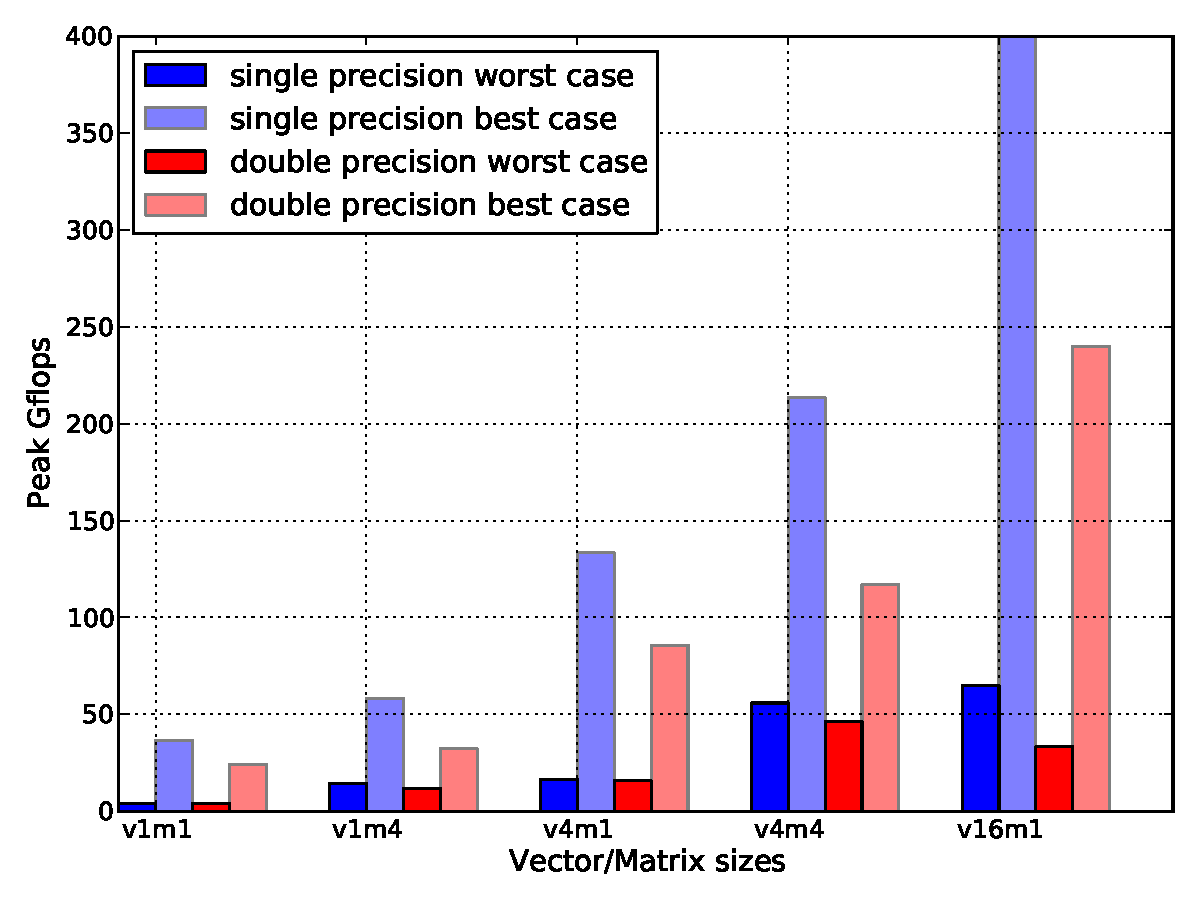
\includegraphics[width=.49\linewidth]{figures/gflops_peak.pdf}\label{fig:gflops_peak_perf}}
%
  \subfigure[Relative performance to base case using one matrix and one
    vector.]{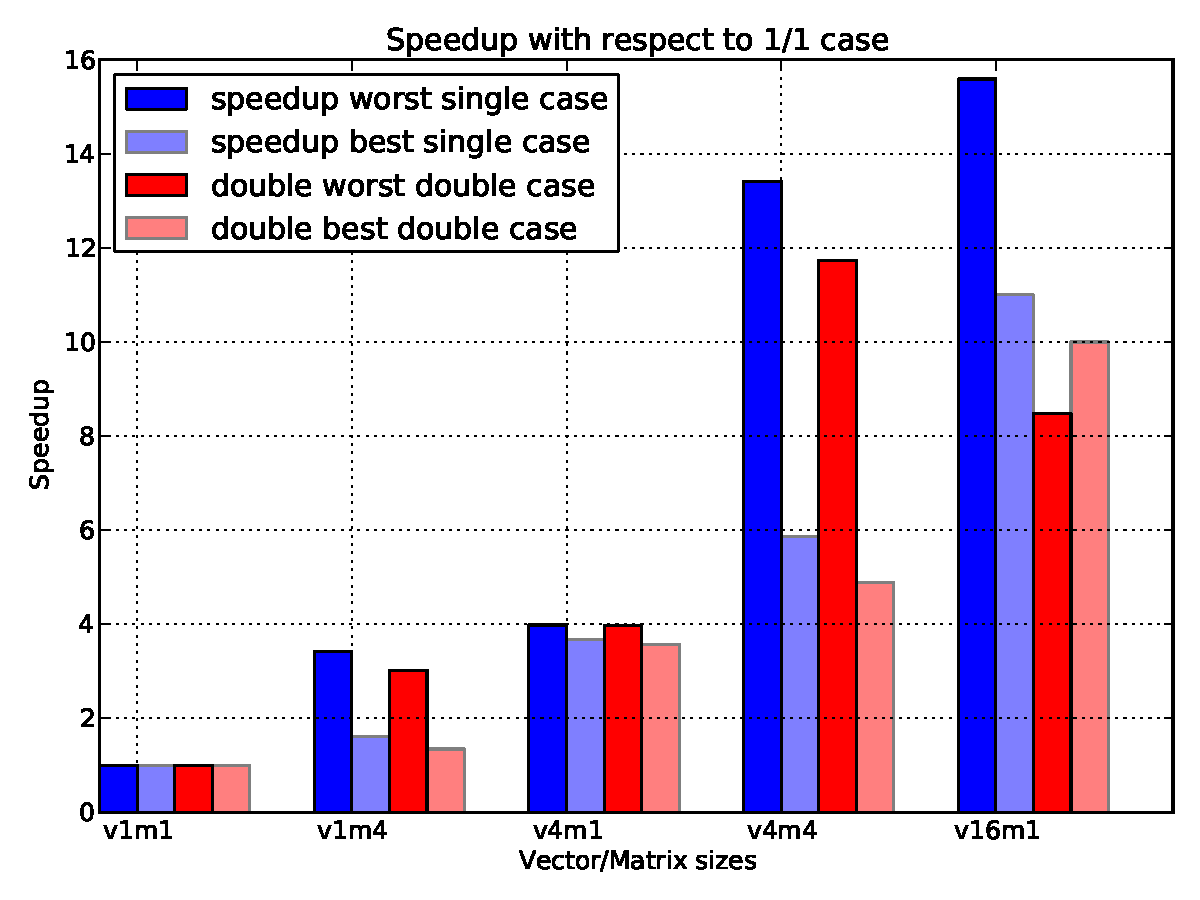
\includegraphics[width=.49\linewidth]{figures/speedup_wrt_base.pdf}\label{fig:speedup}}
  
  \caption{Estimation of the reachable performance one can
      achieve using a device with a memory to computational units of
      150GB/s when varying the number of vectors and matrices}
  \label{fig:perf_predict}
\end{figure*}

\todo{conclude on the evaluation using the figure/table. Note that we
  base prediction on 150GB/s which is not the peak of saule12. Note
  that if you are in best in v1m1 you might go to bad v4m4, but if you
  are in bad v1m1, you will essentially stay there.}

\section{Efficient Implementation on the Intel Xeon Phi processor}
\label{sec:impl}

\subsection{Knights Corner}

In this work, we use an Intel Xeon Phi 5110P coprocessor. This card
has 8 memory controllers where each of them can execute 5 billion
transactions per second and has two 32-bit channels, achieving a total
bandwidth of 320GB/s aggregated across all the memory
controllers. There are 60 cores clocked at 1.05GHz. Their memory
interfaces are 32-bit wide with two channels and the total bandwidth
is 8.4GB/s per core. Thus, the cores should be able to consume 504GB/s
at most. However, the bandwidth between the cores and the memory
controllers is limited by the ring network that connect the cores and
the memory controller. Its precise bandwidth is unknown for this
precise card, but it would be coehrent that it is between 200GB/s and
250GB/s.

Each core in the architecture has a 32kB L1 data cache, a 32kB L1
instruction cache, and a 512kB L2 cache. The architecture of a core is
based the traditional Pentium architecture which have been extended to
64-bit. A core can hold 4 hardware contexts at any time. And at each
clock cycle, instructions from a single thread are executed. Due to
some hardware constraints, two hardware contexts must be used to reach
the peak instruction throughput in that architecture. As in the
Pentium architecture, a core has two different concurrent instruction
pipelines which allow the execution of two instructions per
cycle. However, only one vector or floating point instruction can be
executed at each cycle.

Most of the performance of the architecture comes from the vector
processing unit. Each core has 32 512-bit SIMD registers which can be
used for double or single precision, that is, either as a vector of 8
64-bit values or as a vector of 16 32-bit values, respectively. The
vector processing unit can perform many basic instructions, such as
addition or division, and mathematical operations, such as sine and
sqrt, allowing to reach 8 double precision operations per cycle (16
single precision). The unit also supports Fused Multiply-Add (FMA)
operations which are typically counted as two operations for
benchmarking purposes. Therefore, the peak performance of the 5110P
card is 1 Tflop/s in double precision and 2 Tflop/s in single
precision. If FMA can not be used and half of these number can be
achieved.


\subsection{Bringing the data in vector register}

As explained in Section~XXX, we expect to achieve a performance of
about 210Gflop/s in single precision in the best case. We will focus
on the single precision case with 4 vectors and 4 matrices. But
similar techniques apply for other combinations. This target
performance represents 10\% of the peak performance of the
architecture which is impossible without an efficient vectorization of
the kernel. Indeed, to reach such a performance, a Fused Multiply-Add
instruction on fully loaded registers must be executed at most every
10 cycles.

We discuss how the implementation of the v4m4 kernel works using
vectorial instruction. The code is given for reference in
Figure~\ref{code:mat_mul}. (We will show that an implementation
relying on compiler vectorization does not lead to desirable
performance.) The registers in the MIC architecture are 512 bits wide
and can store 16 floats or integers. (In comparison to OpenCL or CUDA,
one can think of these registers as a warp.) The end goal is to be
able to load and format the non zero values $a,b,c,d$ and the vector
entries $p,q,r,s$ in two vectorial register to be able to apply Fused
Multiply-Add on them, which is depicted in
Figure~\ref{fig:tensor_product}. Bringing the data in the vector
register as depicted in the figure is the difficult part that we now
explain. A thread will perform the multiplications one row at a time,
and parallelism is achieved by giving blocks of rows to each core
usign an OpenMP construct.

\begin{figure}
  \centering
  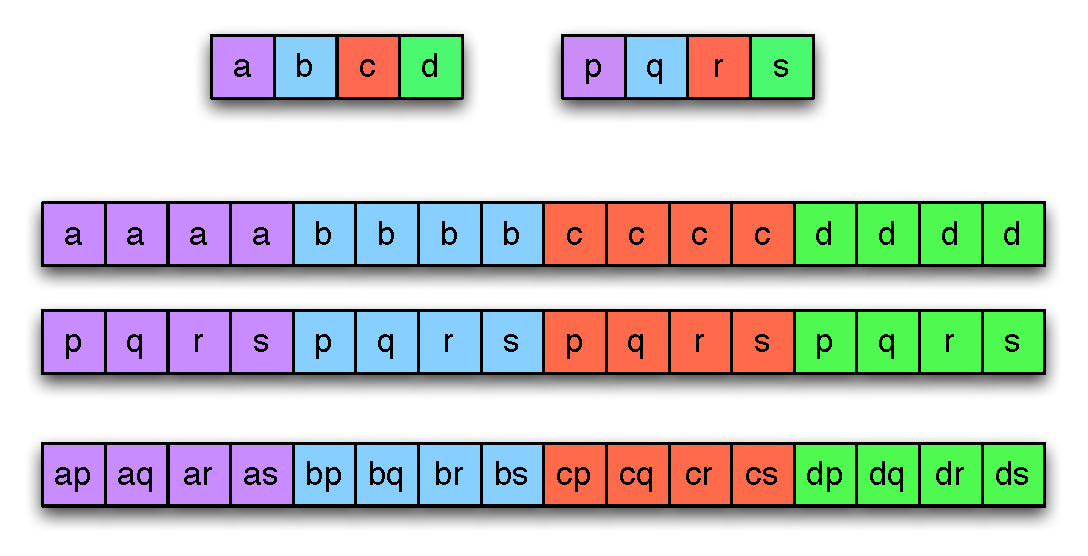
\includegraphics[width=\linewidth]{figures/tensor_product.pdf}
  \caption{Structure of the vector registers to perform an efficient
    tensor scalar product. See Figure~\ref{fig:mat_struct} for
    reference.}
  \label{fig:tensor_product}
\end{figure}

The core of the technique is the use of swizzling and permutation
features of the vectors in the Intel MIC architecture. A vector of 512
bits is composed of 4 lanes (sometimes called channels) of 128 bits
which are made of 4 elements of 32 bits. A swizzling operation allows
to reorder the elements within each lane. While a permutation allow to
change the orders of the lanes. Figure~\ref{fig:swizzling_permutation}
illustrates these two possibilities. Both permutation and swizzling
support common reordering and broadcast. In the code, the ``permute''
function needs to use the {\tt \_mm512\_permute4f128\_epi32}
instruction which is only defined on integers and therefore typecast
are necessary to convert to a vector to/from the integer type.

\begin{figure}
  \centering
  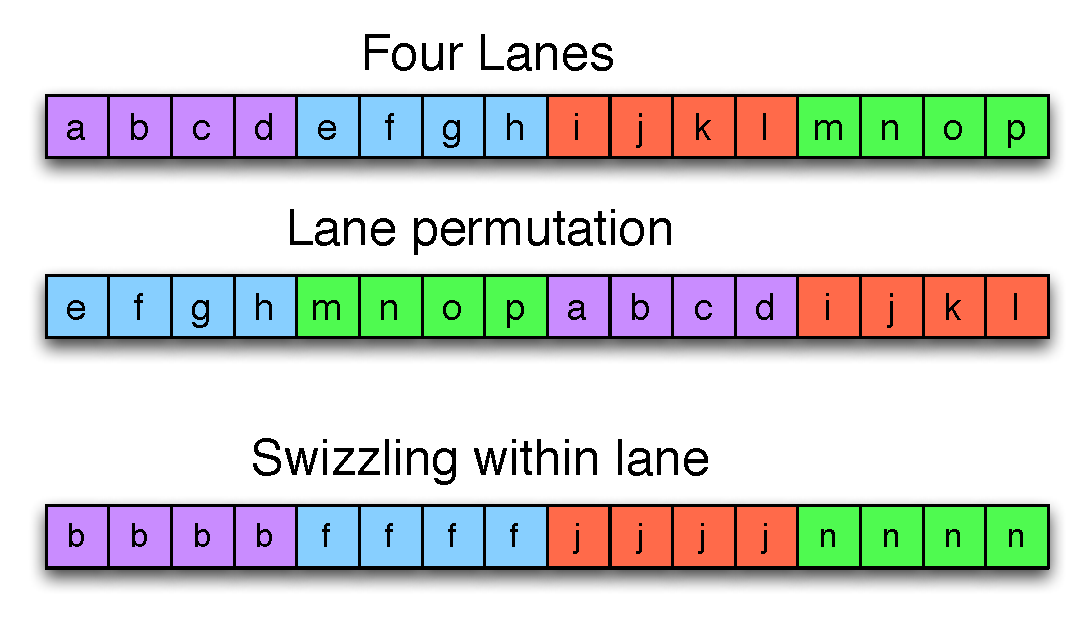
\includegraphics[width=\linewidth]{figures/swizzling_lanes.pdf}
  \caption{Swizzling enables to reorder or broadcast elements within
    each 128 bit group. Permutation enables to reorder or broadcast
    whole 128 bit groups.}
  \label{fig:swizzling_permutation}
\end{figure}

All the operations that loads data from the memory into a register
allows to load 512 bits, so 16 floats at a time. A single non zero in
the matrix will cause 16 operations to be performed, but it only uses
4 floats from the matrix and 4 floats from the {\tt x} vector. So we
need to load at once the data for 4 non zeroes in the matrix, so that
we load 16 flaots from the matrix and 16 floats from the vectors at
once. (The number of non zeroes on a row in our application is always
a multiple of 4, if it was, we would need to add some explicit zeroes
in the data structure to pad it.)

The values from the non zero element in the matrix are the simplest to
load. One can load the 16 floating point values for the 4 non zero of
the matrix at once. The 4 floats coming from the four matrices for
each non zero are naturally grouped within each lane of the SIMD
vector. One can use a swizzle operation to broadcast the 4 elements of
a single matrix to take the whole vector.

Loading the entries from the {\tt x} vector is a little bit more
complicated. First the columns pointers of 4 different non zeroes are
loaded in a vector register and the values are distributed one per
lane of the vector register using an {\tt unpack}
operation\footnote{Notice that there are two calls to unpack for the
  LSB and MSB. Both are mandatory even according the documentation of
  the hardware}. They replicated so that each fill a vector lane using
a swizzle operation. Then each value is multiplied by 4 (because there
are 4 vectors) and the offsets $(3,2,1,0)$ is added each lane to
obtain the correct index of the elements of the {\tt x} vector within
each lane. Then a {\tt gather} operation is performed bring the 16
entries of the {\tt x} vector into the SIMD register. At this point we
have a SIMD register where each lane is the four vector entries for a
non zero element. Using a broadcast permutation, one can replicate an
entry of the four vectors accross each lane.

\begin{figure*}
  \centering
  %\subfigure[Source code}
  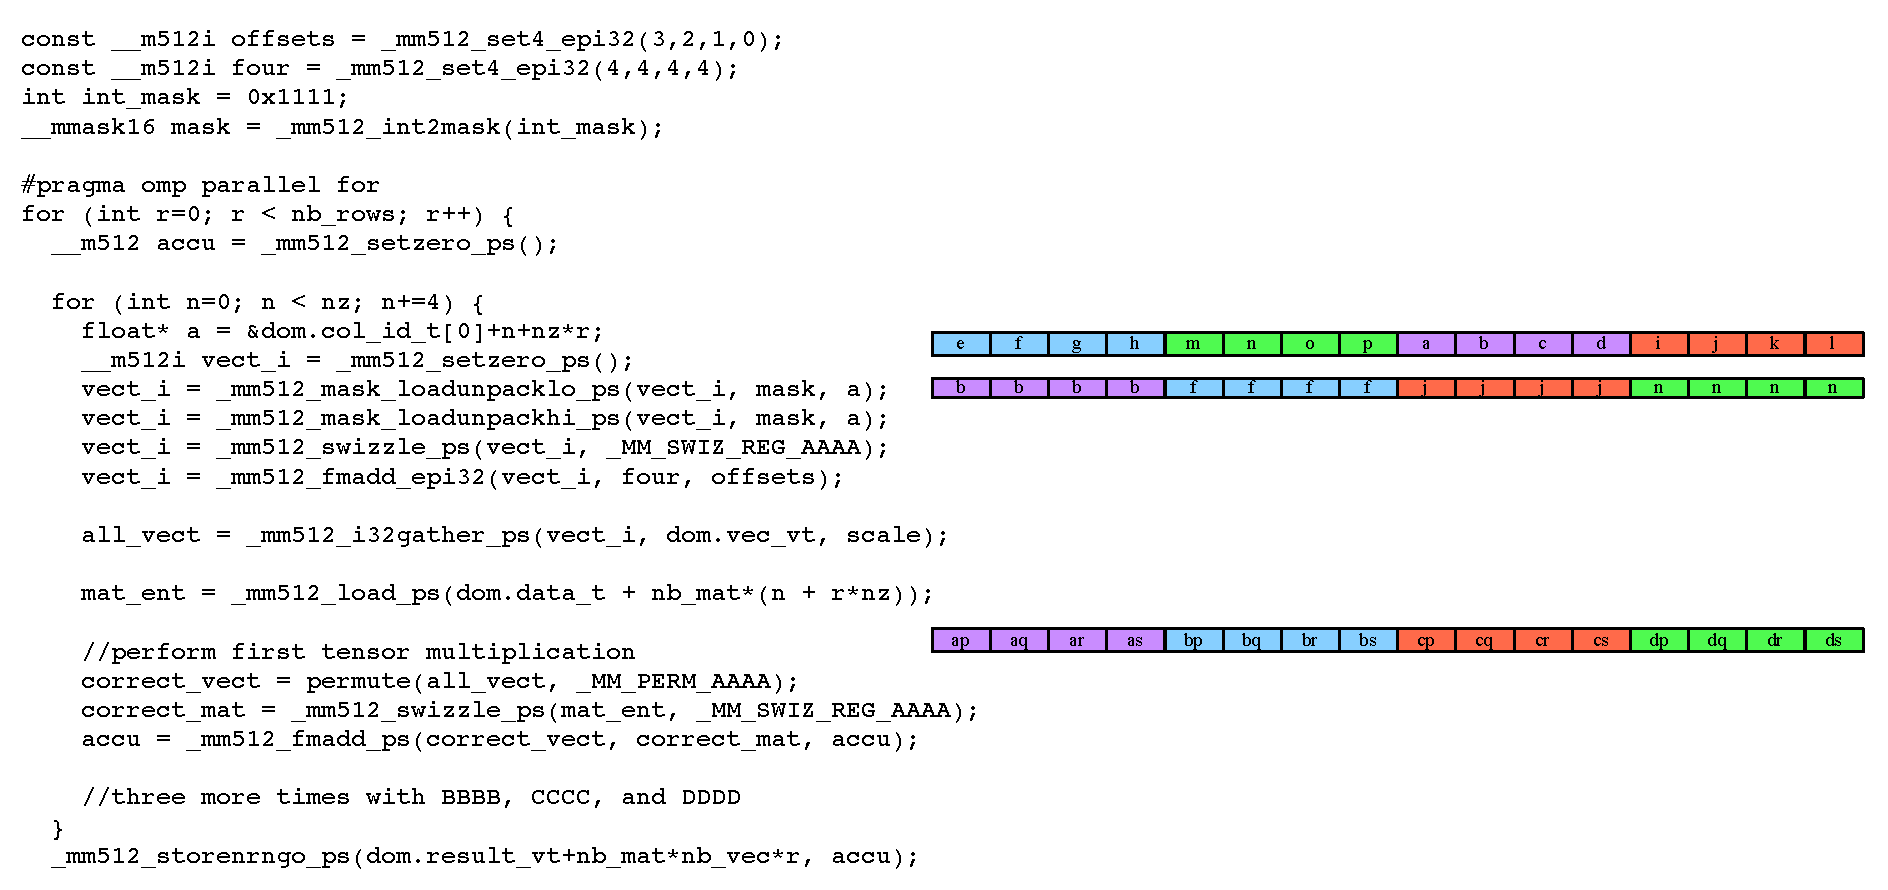
\includegraphics[width=0.8\textwidth]{figures/source_code.pdf}%
  \label{fig:source}
  \caption{Source Code}
\end{figure*}
%\newfig{figures/source_code.pdf}{6in}{Source code}{fig:source}

%\begin{figure}[h]
%\begin{center}
%\lstset{language=c++,basicstyle=\scriptsize,numbers=left,numbersep=5pt}
%\begin{lstlisting}{float=h, Caption}
%const __m512i offsets = _mm512_set4_epi32(3,2,1,0);
%const __m512i four = _mm512_set4_epi32(4,4,4,4); 
%int int_mask = 0x1111;
%__mmask16 mask = _mm512_int2mask(int_mask);
%
%#pragma omp parallel for
%for (int r=0; r < nb_rows; r++) {
%  __m512 accu = _mm512_setzero_ps();
%
%  for (int n=0; n < nz; n+=4) {
%    float* a = &dom.col_id_t[0]+n+nz*r;
%    __m512i vect_i = _mm512_setzero_ps();
%    vect_i = _mm512_mask_loadunpacklo_ps(vect_i, mask, a);
%    vect_i = _mm512_mask_loadunpackhi_ps(vect_i, mask, a);
%    vect_i = _mm512_swizzle_ps(vect_i, _MM_SWIZ_REG_AAAA);
%    vect_i = _mm512_fmadd_epi32(vect_i, four, offsets);
%
%    all_vect = _mm512_i32gather_ps(vect_i, dom.vec_vt, scale);
%
%    mat_ent = _mm512_load_ps(dom.data_t + nb_mat*(n + r*nz));
%
%    //perform first tensor multiplication
%    correct_vect = permute(all_vect, _MM_PERM_AAAA);
%    correct_mat = _mm512_swizzle_ps(mat_ent, _MM_SWIZ_REG_AAAA);
%    accu = _mm512_fmadd_ps(correct_vect, correct_mat, accu);
%
%    //three more times with BBBB, CCCC, and DDDD
%  }
%  _mm512_storenrngo_ps(dom.result_vt+nb_mat*nb_vec*r, accu);  
%\end{lstlisting}
%\end{center}
%\end{figure}
%




%\begin{figure*}
%\begin{verbatim}
%const __m512i offsets = _mm512_set4_epi32(3,2,1,0);
%const __m512i four = _mm512_set4_epi32(4,4,4,4); 
%int int_mask = 0x1111;
%__mmask16 mask = _mm512_int2mask(int_mask);
%
%#pragma omp parallel for
%for (int r=0; r < nb_rows; r++) {
%  __m512 accu = _mm512_setzero_ps();
%
%  for (int n=0; n < nz; n+=4) {
%    float* a = &dom.col_id_t[0]+n+nz*r;
%    __m512i vect_i = _mm512_setzero_ps();
%    vect_i = _mm512_mask_loadunpacklo_ps(vect_i, mask, a);
%    vect_i = _mm512_mask_loadunpackhi_ps(vect_i, mask, a);
%    vect_i = _mm512_swizzle_ps(vect_i, _MM_SWIZ_REG_AAAA);
%    vect_i = _mm512_fmadd_epi32(vect_i, four, offsets);
%
%    all_vect = _mm512_i32gather_ps(vect_i, dom.vec_vt, scale);
%
%    mat_ent = _mm512_load_ps(dom.data_t + nb_mat*(n + r*nz));
%
%    //perform first tensor multiplication
%    correct_vect = permute(all_vect, _MM_PERM_AAAA);
%    correct_mat = _mm512_swizzle_ps(mat_ent, _MM_SWIZ_REG_AAAA);
%    accu = _mm512_fmadd_ps(correct_vect, correct_mat, accu);
%
%    //three more times with BBBB, CCCC, and DDDD
%  }
%  _mm512_storenrngo_ps(dom.result_vt+nb_mat*nb_vec*r, accu);  
%} 
%\end{verbatim}
%\caption{mat mul code.}
%\label{code:mat_mul}
%\end{figure*}





\section{Experimental Validation}
\label{sec:expe}

\subsection{Instances}


\def\ww{.13\textwidth}
\begin{figure*}
  \begin{center}
    \subfigure[Supercompact.]{%
      \label{fig:supercompact}
      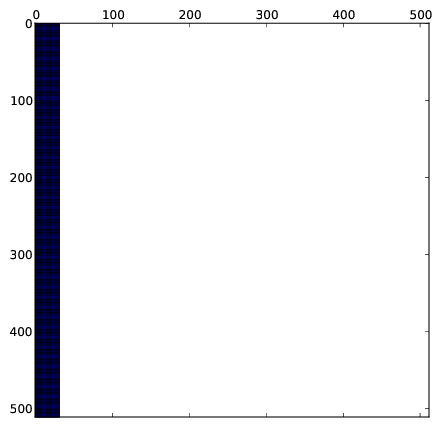
\includegraphics[width=\ww]{figures/supercompact_matrix-crop.png}}%
    \subfigure[Compact.]{%
      \label{fig:compact}
      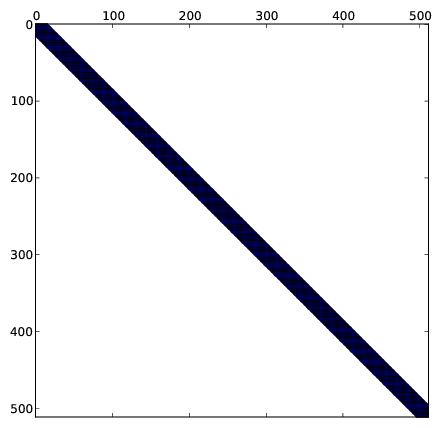
\includegraphics[width=\ww]{figures/compact_matrix-crop.png}}%
    \subfigure[Random.]{%
      \label{fig:random}
      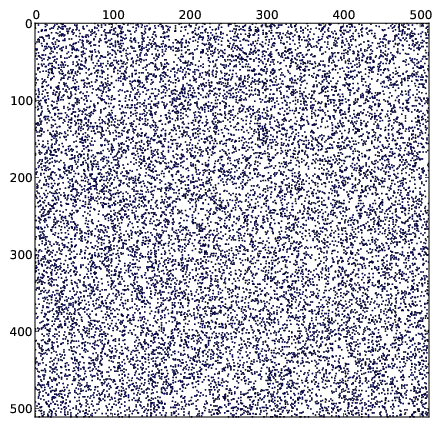
\includegraphics[width=\ww]{figures/random_matrix-crop.png}}%
    \subfigure[2D, no RCM.]{%
      \label{fig:rbf2dnorcm}
      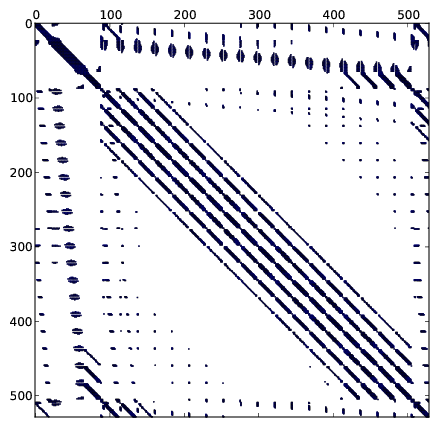
\includegraphics[width=\ww]{figures/kd-tree-2d-norcm-crop.png}}%
    \subfigure[2D, RCM.]{%
      \label{fig:rbf2drcm}
      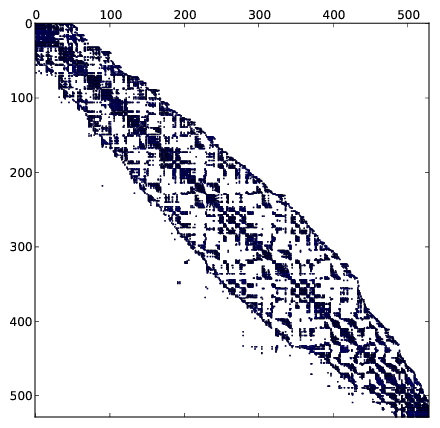
\includegraphics[width=\ww]{figures/kd-tree-2d-rcm-crop.png}} 
    \subfigure[3D, RCM.]{%
      \label{fig:rbf3dnorcm} 
      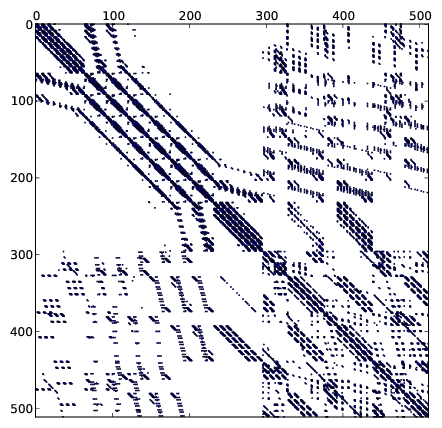
\includegraphics[width=\ww]{figures/kd-tree-3d-norcm-crop.png}}%
    \subfigure[3D, RCM.]{%
      \label{fig:rbf3drcm}
      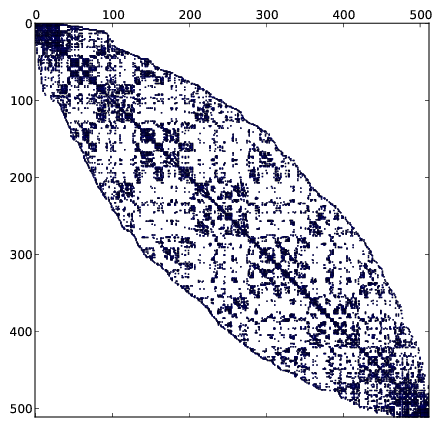
\includegraphics[width=\ww]{figures/kd-tree-3d-rcm-crop.png}}%
  \end{center}
  
  \caption{Different sparsity distributions. In all cases, there are
    32 nonzeros per line and 300 rows. The last four matrices
    corresponds to derivative stencils in 2D and 3D RBF-FD
    calculations.}
  \label{fig:spy_plots}
\end{figure*}

To perform our experiments and analysis, we use multiple kinds of
matrices which are presented in Figure~\ref{fig:spy_plots}. The
Supercompact matrices (Figure~\ref{fig:supercompact}) have been
generated to only have non zero elements in the first 32 columns of
the matrix. That way we ensure the simplest form of multiplication,
the amount of elements from the {\tt x} vector data transfered from
the memory will be minimum. The Compact matrices
(Figure~\ref{fig:compact}) are generated to have 32 non zeroes per row
centered around the diagonal and it represents the ideal case for most
application relying on sparse matrix vector multiplication. The Random
matrices (Figure~\ref{fig:compact}) see their non zero element
randomly (uniformly) distributed in the matrix, they represent the
worst case scenario for cache based architecture where the cache
reutilisation is the lowest from one row to the next.

The other two types of matrices are used in derivative stencils in 2D
and 3D RBF-FD calculations (Figure~\ref{fig:rbf2dnorcm} pictures a
$32$-points stencil of a $23^2$ 2D grid and
Figure~\ref{fig:rbf2dnorcm} shows a $32$-points stencil of a $8^3$
grid). We also apply Cuthill-Mckee reordering to all the matrices This
ordering technique is designed to reduce the distance between the non
zeroes and the diagonal, hopefully allowing a better cache
reutilisation. The reordered version of these two matrices can be seen
in Figure~\ref{fig:rbf2drcm} and in Figure~\ref{fig:rbf3drcm}.


\subsection{Bandwidth}

\begin{figure*}
\centering
  \subfigure[
    Entries with "cpp" denote cases where
    coding was performed without MIC vector
    instructions.]{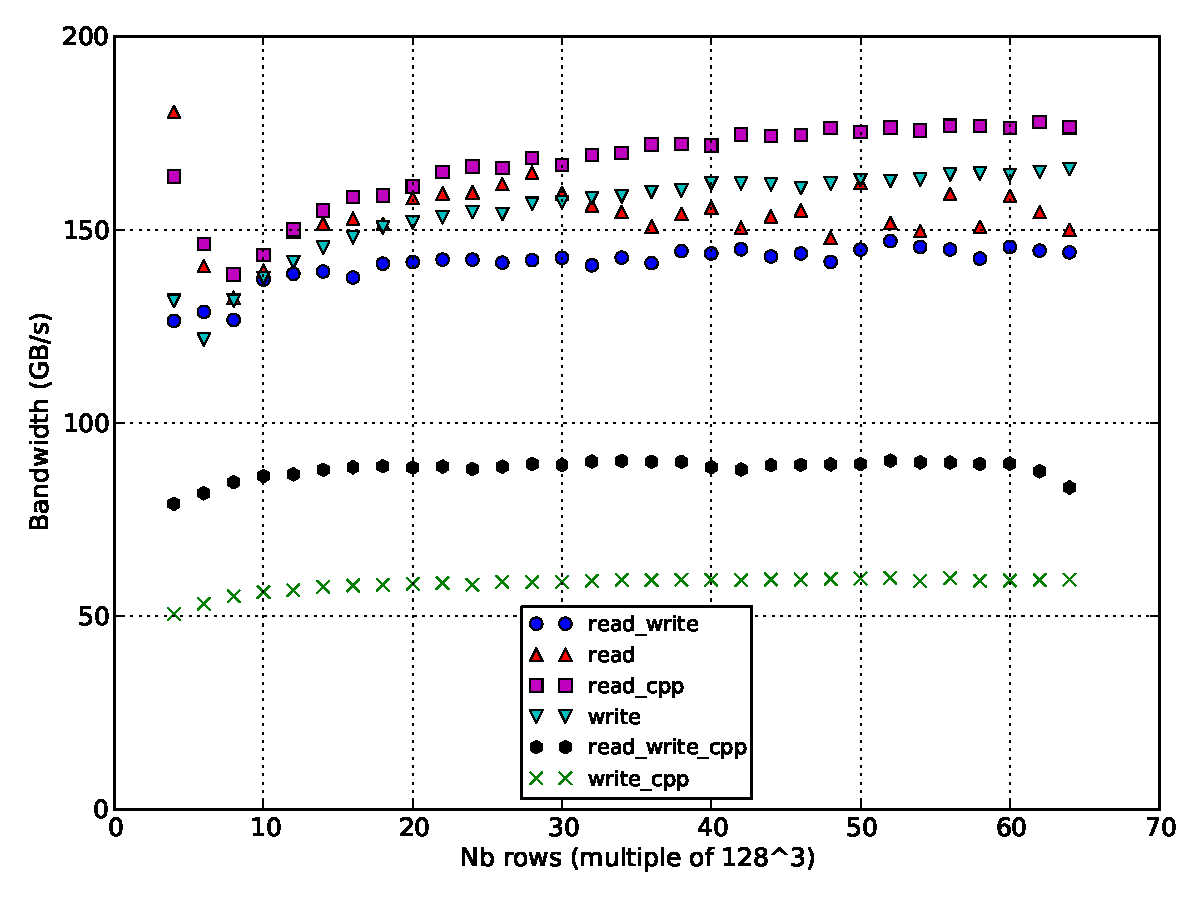
\includegraphics[width=.40\linewidth]{figures/test1_readwrite.pdf}\label{fig:band_rw}}
%
  \subfigure[ xxx ] 
  {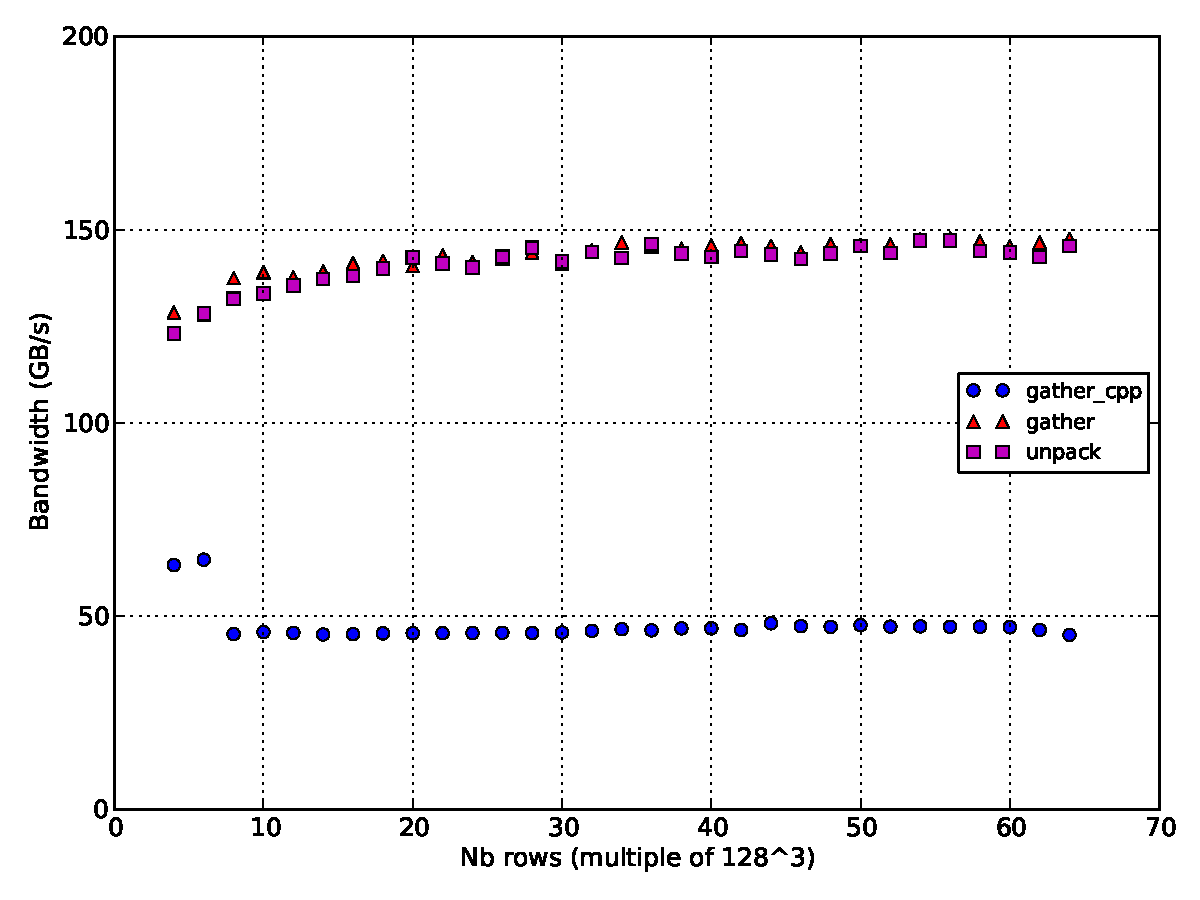
\includegraphics[width=.40\linewidth]{figures/test1_gather.pdf}\label{fig:band_gather}} \\

  \subfigure[The greater
    speed of the cpp version is obtained throught the use of
    \ttt{\#Ivdep} {\em and\/} \ttt{\_\_assumed\_aligned}. All memory
    is aligned on 64
    bytes.]{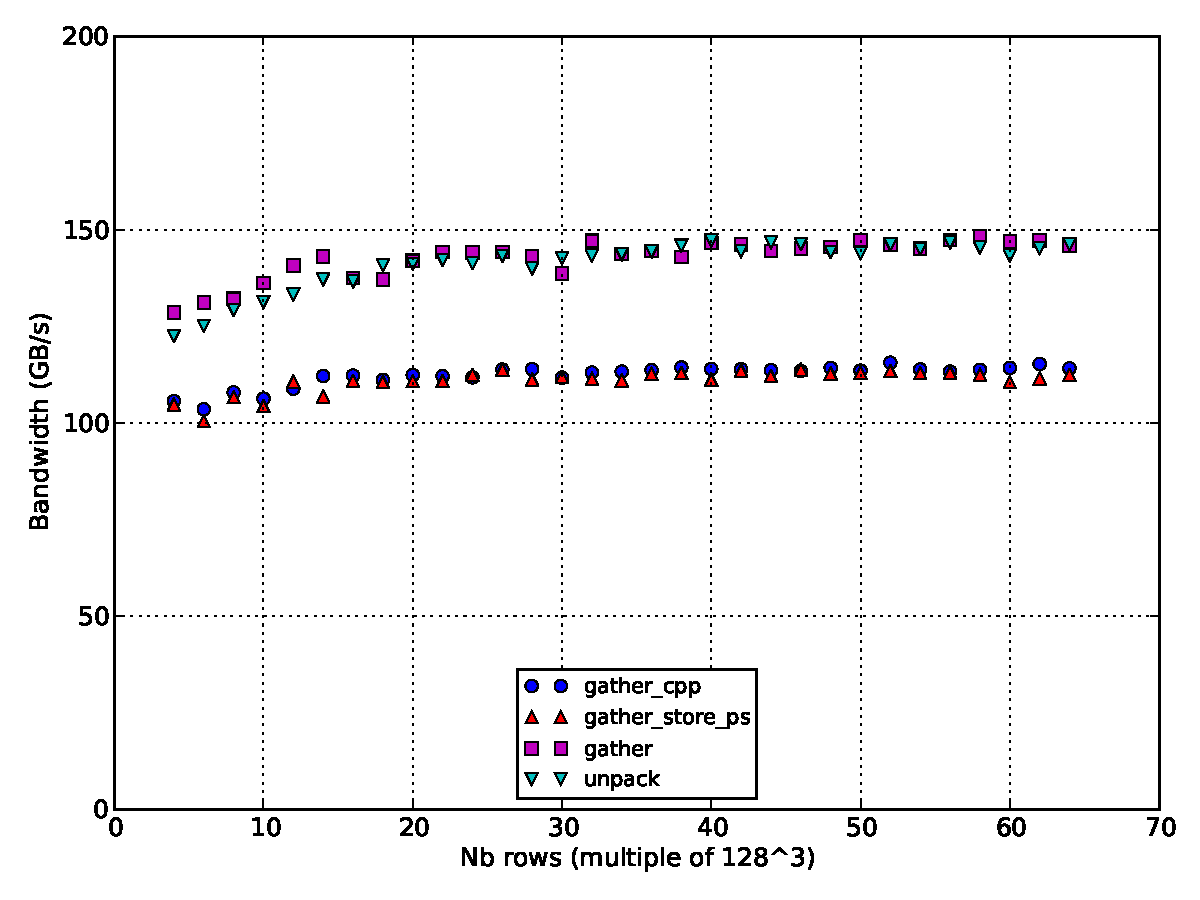
\includegraphics[width=.40\linewidth]{figures/test3_gather.pdf}\label{fig:band_gather_ivdep}}
%
  \subfigure[
    The speed on the CPU matches the speed with vector instructions.
    All memory is aligned on 32
    bytes.]{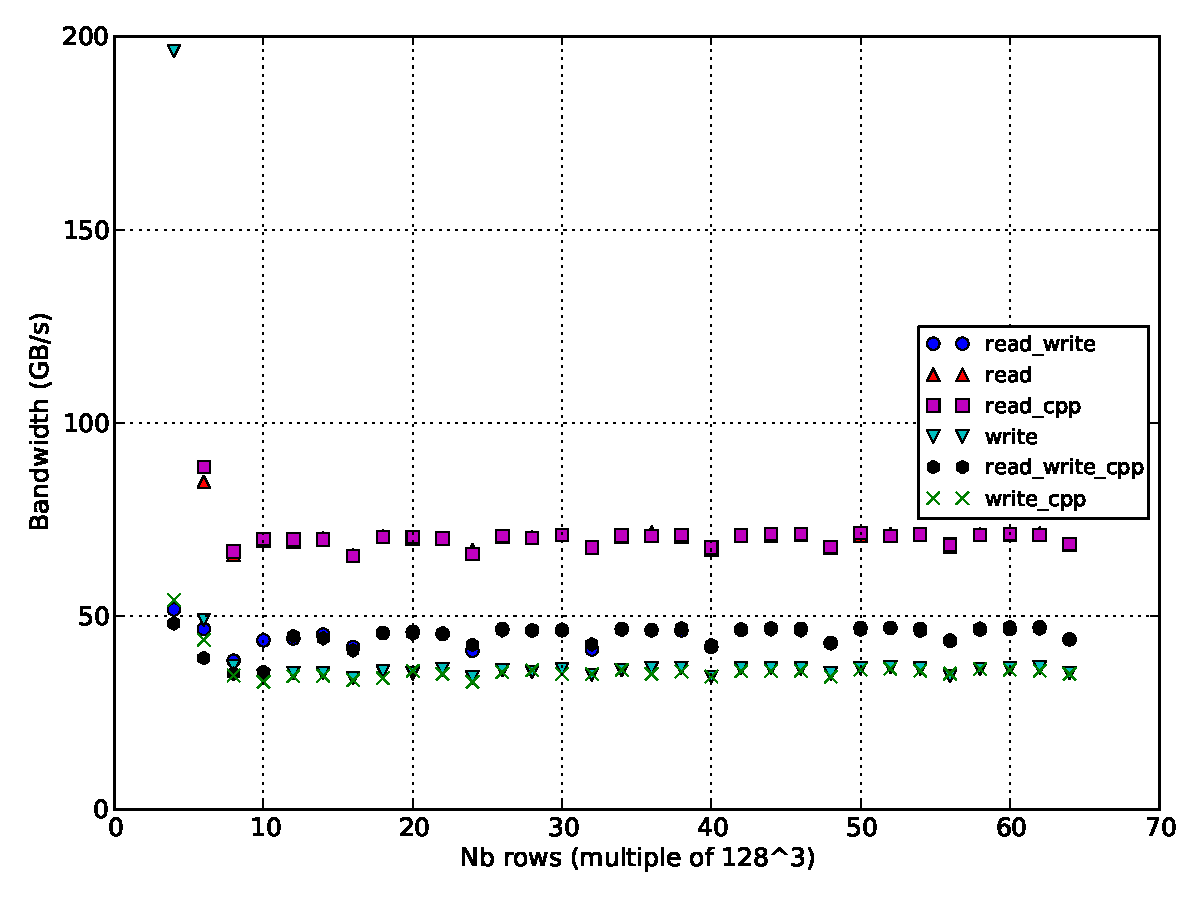
\includegraphics[width=.40\linewidth]{figures/host_test1_readwrite_no_temporal_hint.pdf}\label{fig:read_write}}

\caption{Bandwidth performance on the host under idealized conditions as a function of matrix row size.
  Entries with "cpp" denote cases where coding was performed without MIC vector intructions. 
\todo{not 100\% sure what this plots are.}}
\end{figure*}

\subsection{Computations}

\begin{figure*}
  \centering
  \subfigure[Performance of $y=Ax$ on the MIC. Squares: base 1/1 case,
    solid circles: 4/4 case implemented in C++, solid triangles: 4/4
    case implemented with MIC vector instructions. $-O3$ compilation
    options. Each symbol has two cases: with (red) and without blue) 
    with and without Reverse Cuthill-McKee. The grid is $96^3$.]
    {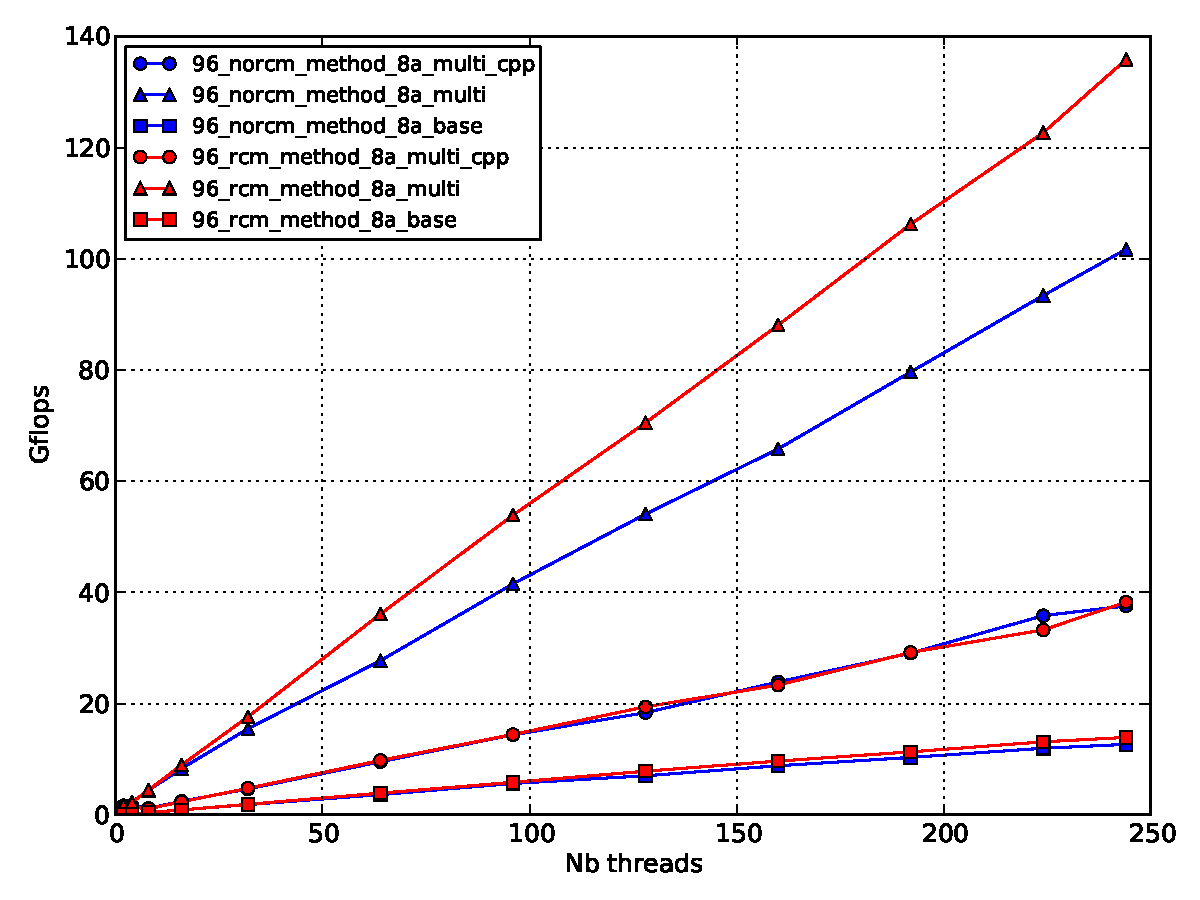
\includegraphics[width=.40\linewidth]{figures/mic_performance_nb_threads.pdf}\label{fig:perf_mic}}
%
  \subfigure[Performance on the host on a sparse matrix with $64^3$ rows. Manual
    vectorization brings significant improvement there as
    well.]{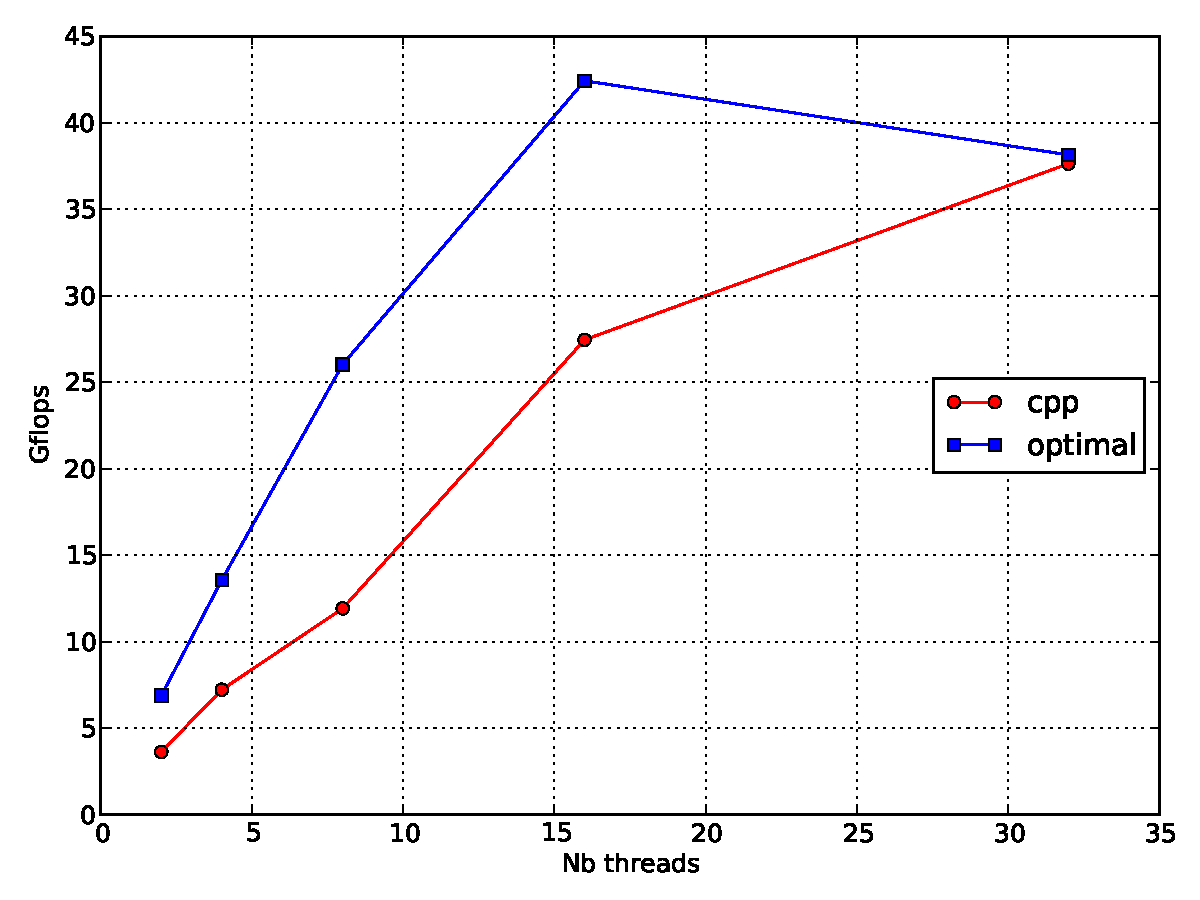
\includegraphics[width=.40\linewidth]{figures/64x64x64.pdf}\label{fig:perf_host}}
  \caption{Vectorization matters in practice. Differences in BW
    translate in different performance.\todo{this two plots should ``correlate'' }}
\end{figure*}


\begin{figure}[t]
  \centering
  \subfigure[Supercompact]{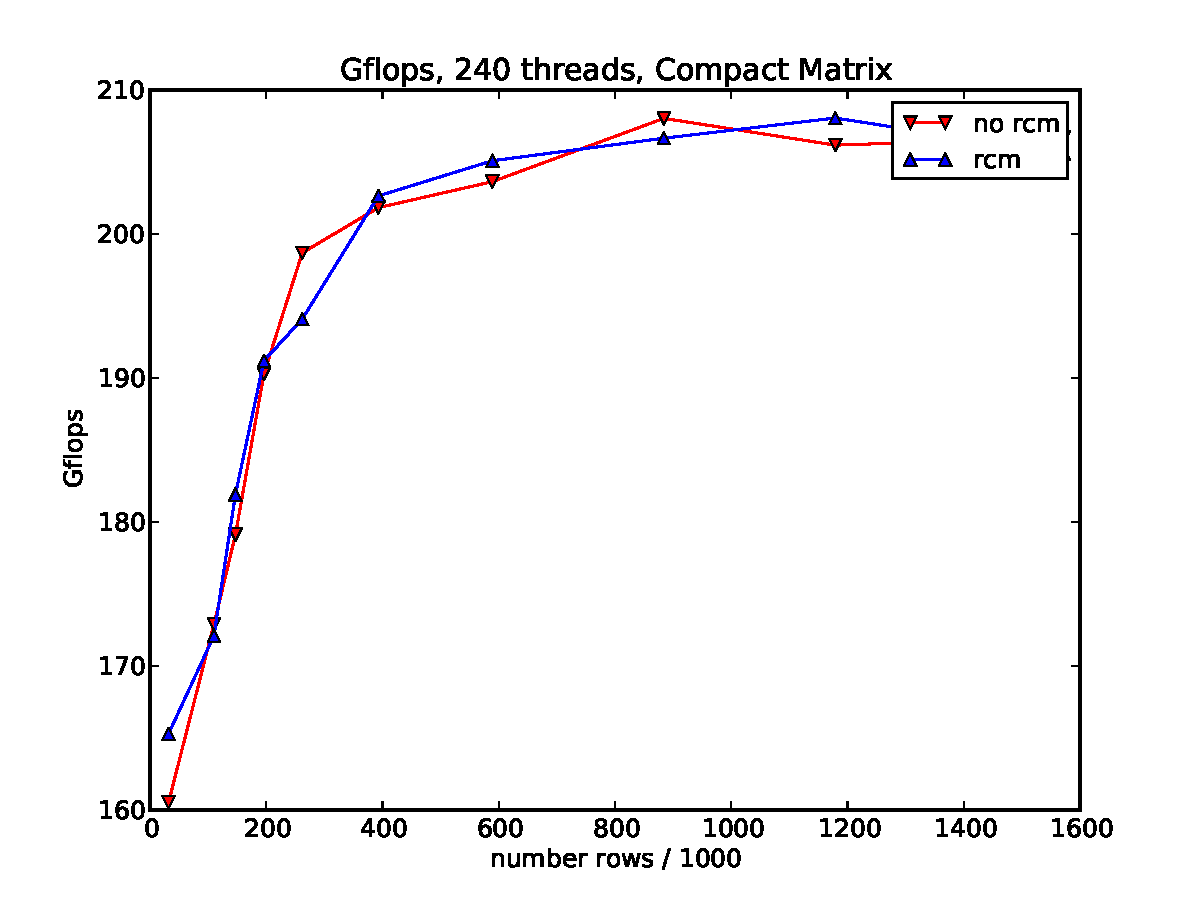
\includegraphics[width=.48\linewidth]{figures/supercompact_max_perf.pdf}}
  \subfigure[Compact]{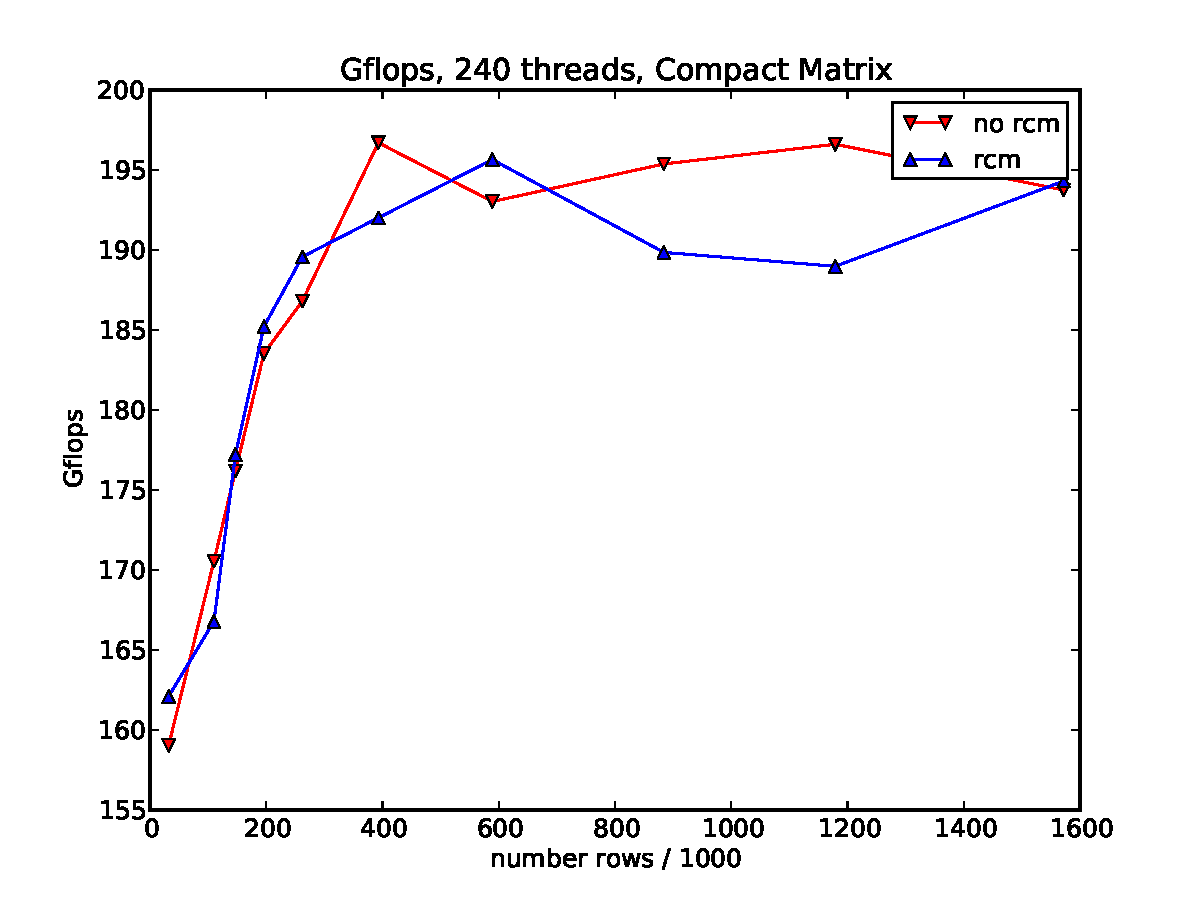
\includegraphics[width=.48\linewidth]{figures/compact_max_perf.pdf}} \\
  \subfigure[Random]{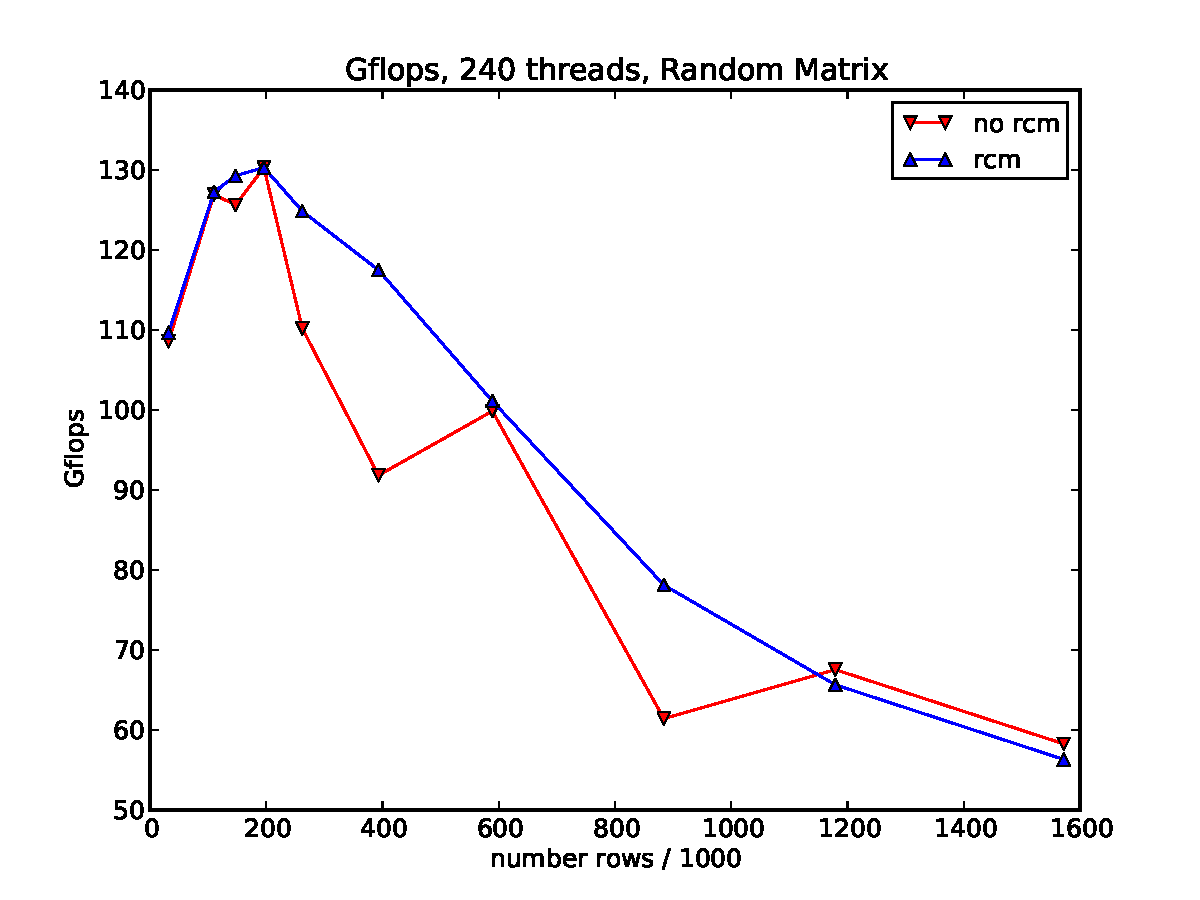
\includegraphics[width=.48\linewidth]{figures/random_max_perf.pdf}}
  \subfigure[RBF 3D]{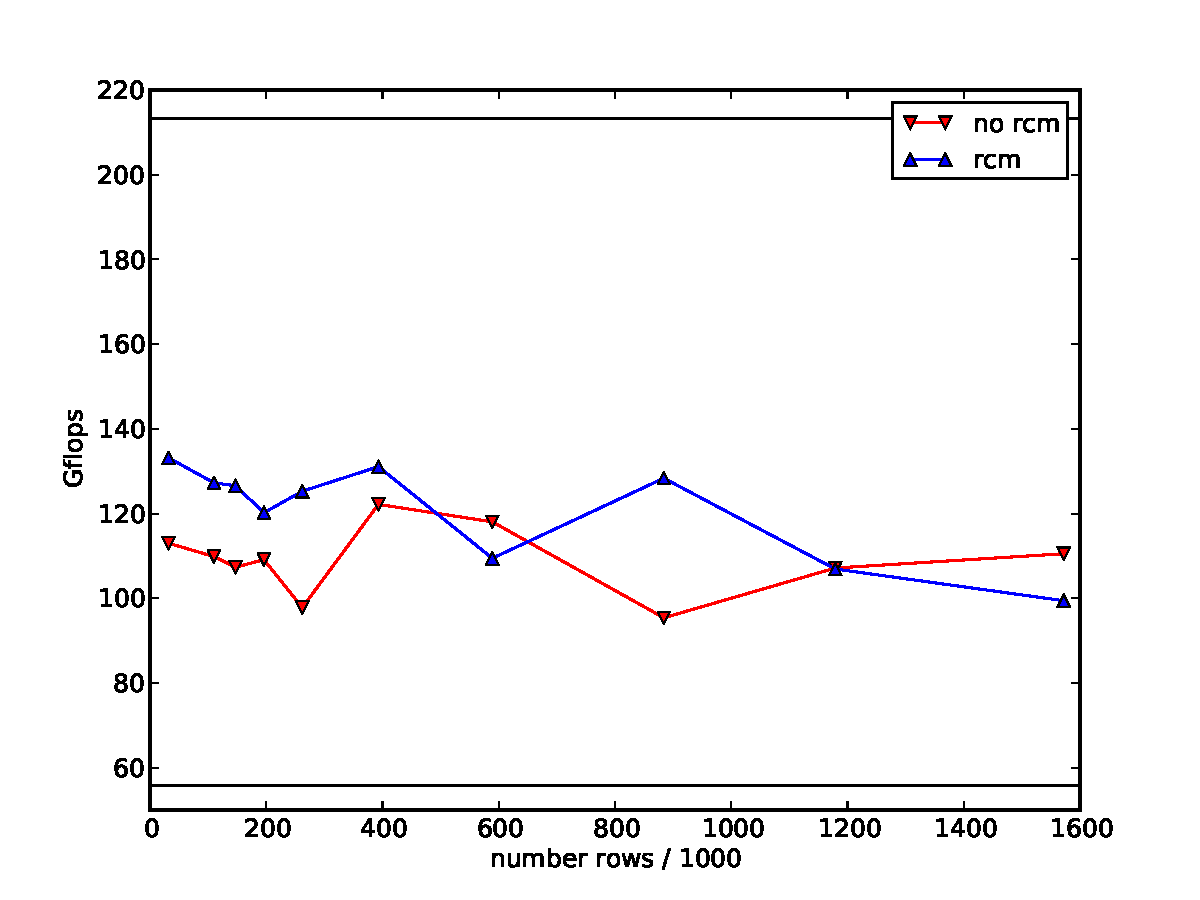
\includegraphics[width=.48\linewidth]{figures/rbf_max_perf_run1.pdf}}
  \caption{Performance of "best code" accross instance types. \todo{Why stop at 1.6M
      rows. Is that because of memory limitation? I guess that's what
      it is}}
\end{figure}


\begin{figure}
  \centering
  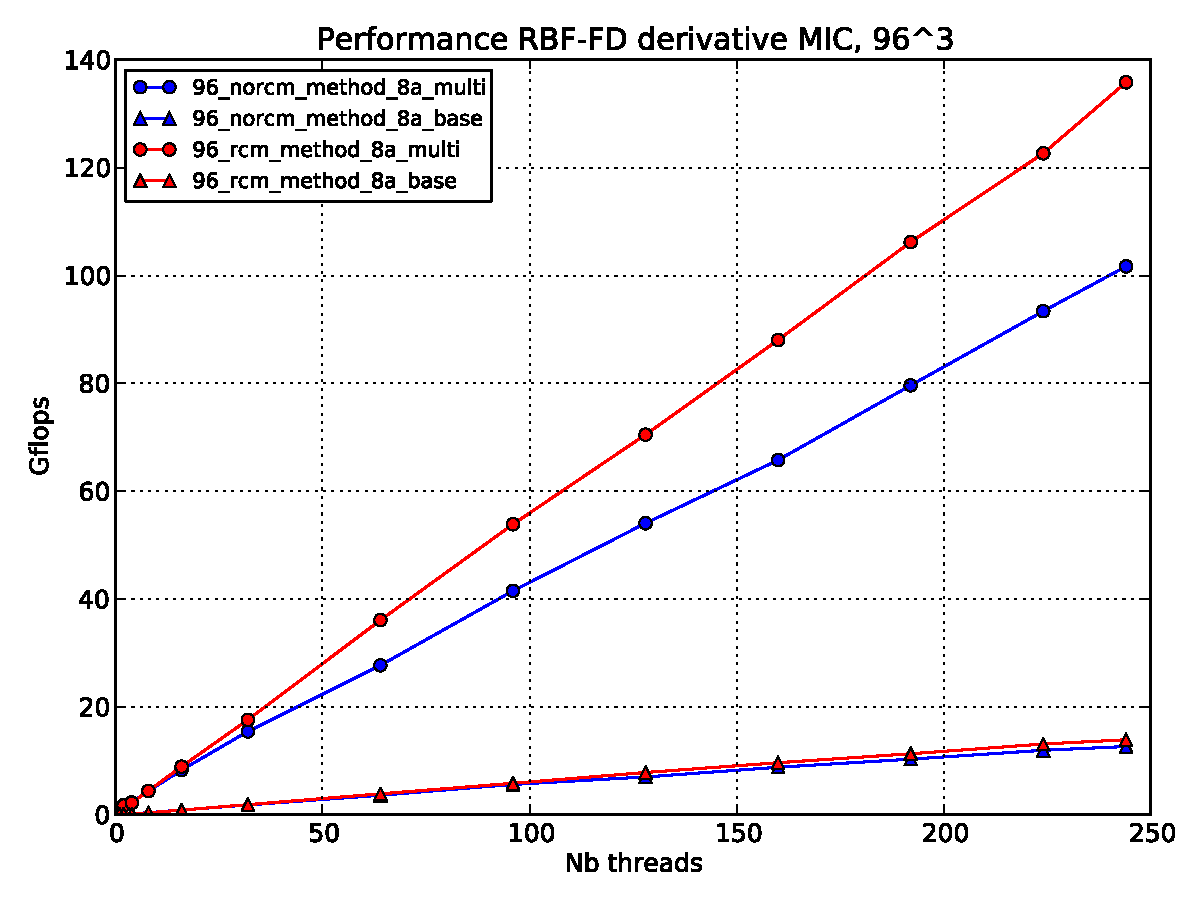
\includegraphics[width=.45\textwidth]{figures/plot_for_natasha_ncar_end_of_year.pdf}

  \caption{Performance on a MIC of derivative computation for RBFFD
    with 884,736 nodes distributed quasi-randomly in a cube. Single
    derivative of a single function (base case, triangle) and four
    derivatives of four functions (multi case, circles). No bandwidth
    reduction (blue) and Reverse Cuthill-McKee (red).\todo{should we have a similar one for the host?}}
\end{figure}

\begin{figure*}
\centering
\subfigure[Best case.]{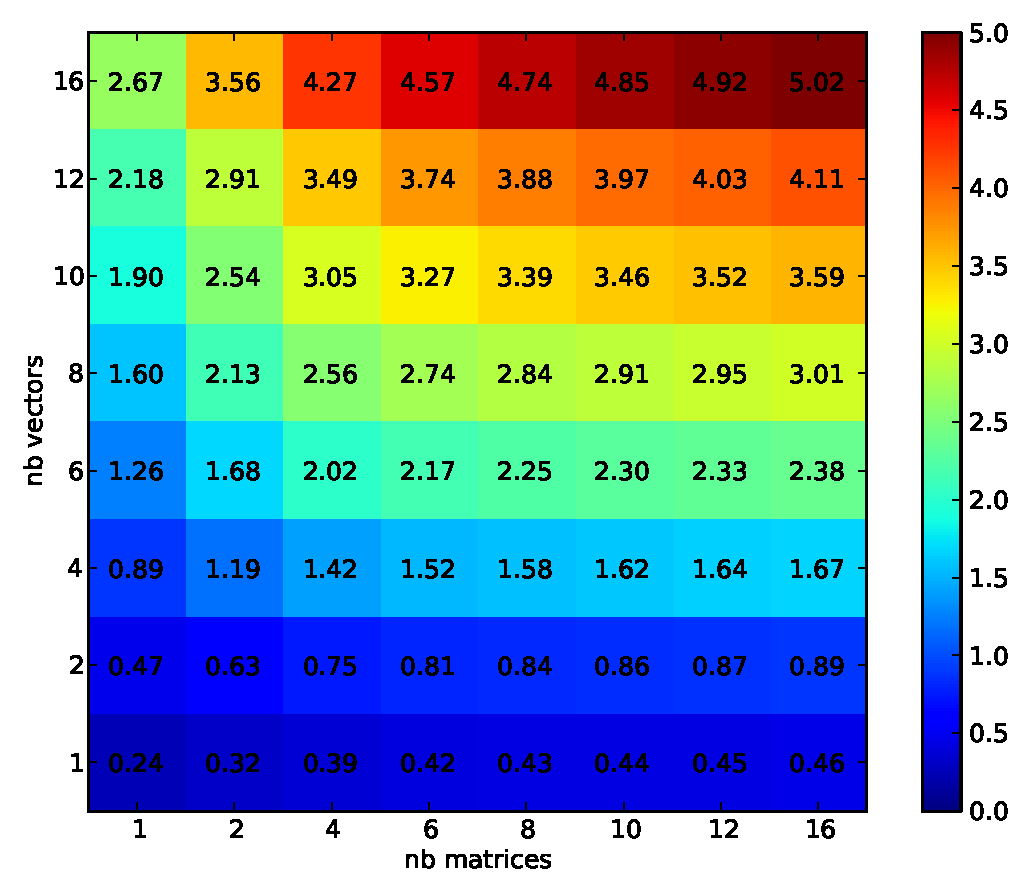
\includegraphics[width=.33\linewidth]{figures/flops_to_bytes_best-crop.pdf}} %\label{fig:ratio_best}}
\subfigure[Worst case.]{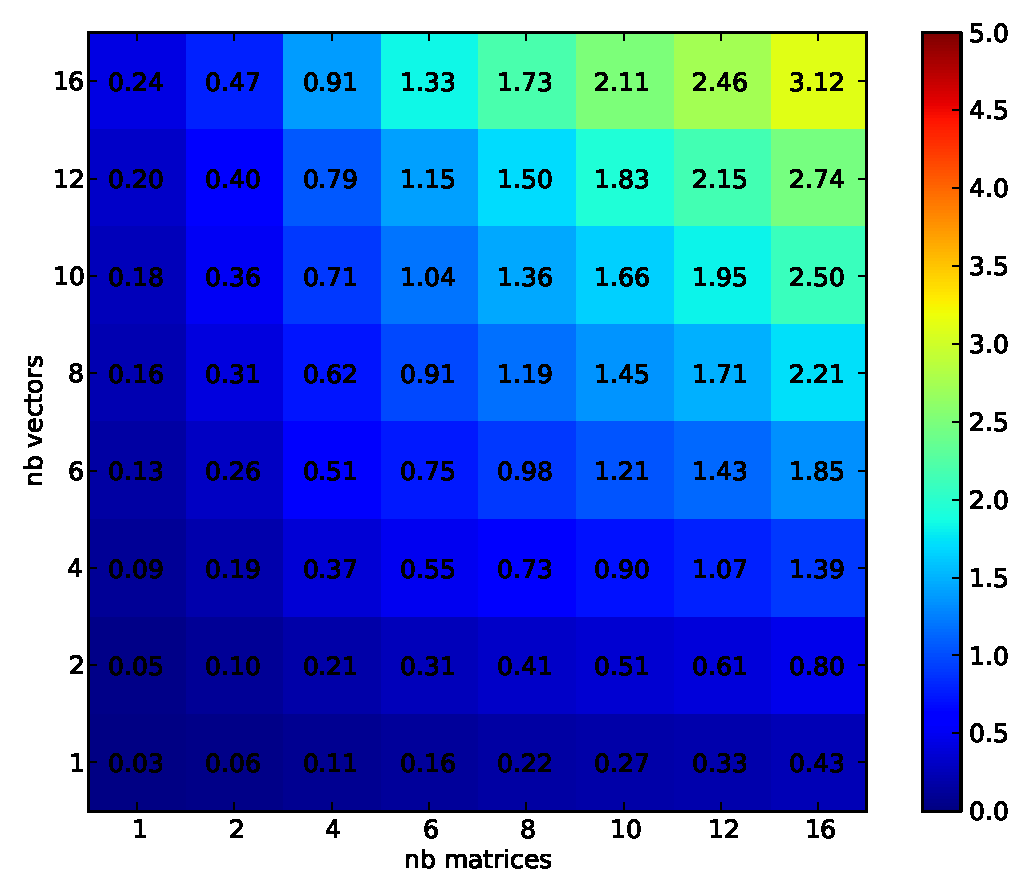
\includegraphics[width=.33\linewidth]{figures/flops_to_bytes_worst-crop.pdf}}%\label{fig:ratio_worst}}
\subfigure[Worst case (No cacheline effects)]{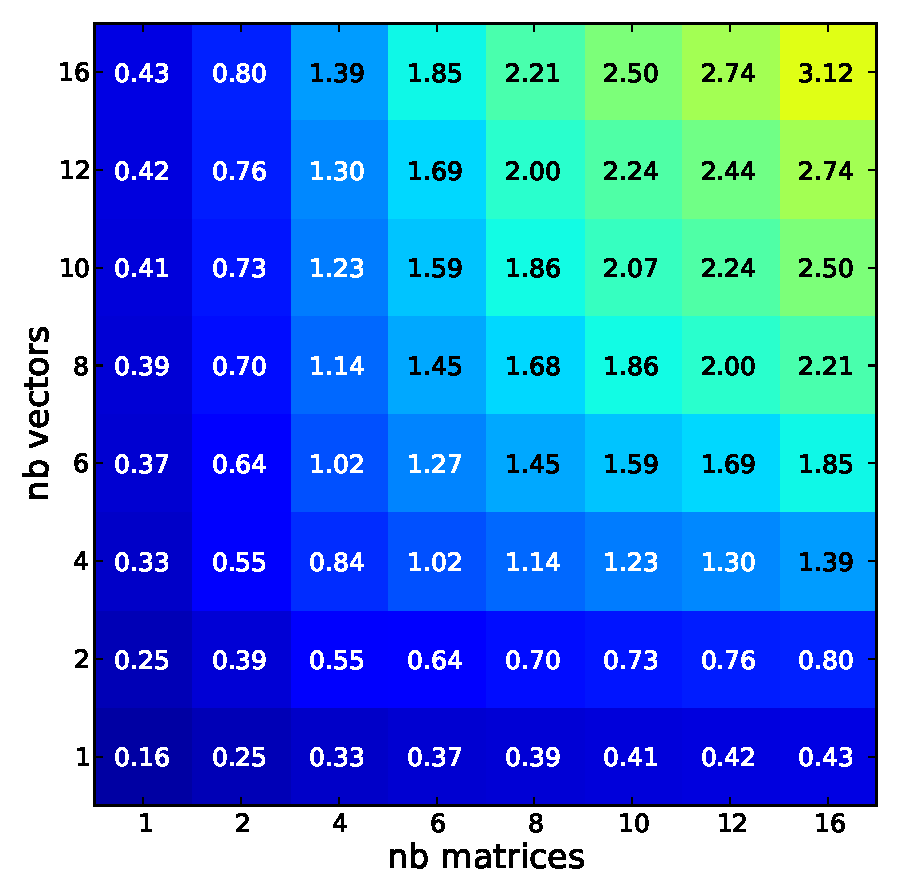
\includegraphics[width=.33\linewidth]{figures/flops_to_bytes_no_cache-crop.pdf}}%\label{fig:ratio_nocache}}
\caption{Ratio of flops to bytes; (a) simple count of flops and bytes that require transfer from memory;(b) best and (c) worst
case taking into account that bringing one element of $x$ into memory brings along the remainder of the cache line.}
\label{fig:ratio_bytes_flops}
\end{figure*}

Derivatives in an RBFFD formulation are expressed as a sparse
matrix/vector multiplication (SpMV). Using the full 61 nodes of a MIC
processor, and all four threads of each node, we achieve lowly 18
Gflops when calculating a single vector of a single
function. Bandwidth reduction has minimal effect since the cache is
large enough to store both the derivative matrix and the solution
vector. We increase the number of computations per byte transferred by
calculating four different derivatives of four different
functions. With bandwidth reduction, we speed the calculation by a
factor of 8, and achieve upwards of 140 Gflops.


\section{Conclusion}
\label{sec:ccl}

In the previous sections, we have explored in the practical
implementation on a MIC architecture of multiple derivative operators
acting on multiple vectors within the context of RBF-RD. Each
derivative has an associated sparse matrix with a fixed number of
non-zeros on each row. While computing a single derivative of multiple
functions is rather common (vectorization occurs over the vectors), we
accelerate the algorithm further by considering multiple derivatives
with corresponding matrices with identical adjacency graphs. We
specialize to four matrices and four derivatives, with 16 outputs,
computed as a sum of outer products.

Using a matrix with $64^3$ (or $96^3$ rows, we achieve a speedup of
xxx relative to the base case of one derivative and one function (1/1
case), relative to a potential speedup of 16. We have achieved a
speed of 100 Gflop/s on 60 cores using 240 threads, or a speed of 61\% of
maximum possible performance. The maximum possible speed for the 1/1
case is around 40 Gflop/s, of which we achieve 20 Gflop/s. On matrices
that exceed the cache, a reverse Cuthill-McKee is applied to reduce the
bandwidth, with an associated speedup of 30\% up to 135 Gflop/s. Our
optimal implementation makes use of the (as yet unreleased) IMCI MIC instruction set 
%\todo{that's not AVX on MIC, not sure what the name is}, 
which includes a number of swizzling and channel swapping operations, for an
extremely efficient tensor product implementation. A straightforward
implementation without vectorization runs at around 35 Gflops, or 16\% of peak
performance. RCM has no effect because the number of floating point
operations is excessive (the algorithm does not fill the vector
registers to capacity).

In a future work, we will examine the effect of larger stencil sizes,
double precision, and the actual cost of computing the derivatives
within a fluid simulation using RBF-FD.

\section*{Acknowledgment}
The first and last authors acknowledge NSF funding under NSF grant DMS-\#0934331 (FSU). 
NCAR is sponsored by the National Science Foundation. N. Flyer      
acknowledges support of NSF grant DMS-0934317.


\bibliographystyle{plain} %{IEEEabrv,paper.bib}
\bibliography{paper, bollig}
\end{document}


